\chapter{Finite element spaces}

\disclaimer

\section{Introduction}
The objective of this section is threefold.  We first introduce finite elements for reference triangles. We then discuss the assembly of finite elements to construct a finite element space.  We finally discuss approximation properties of these finite element spaces.

\section{Triangulation}
We first introduce a \emph{triangulation} of $\Omega \subset \RR^d$.  A triangulation
\begin{equation*}
  \calT_h \equiv \{ K_i \}_{i=1}^{n_e}
\end{equation*}
is a set of non-overlapping elements $K_1, \dots, K_{n_e}$ such that union of the closure of the elements cover the domain: $\cup_{i=1}^{n_e} \overline K_i = \overline \Omega$.   (We consider the closure of the elements because we consider each element to be open.) An example of triangulation of a square domain $\Omega$ is shown in Figure~\ref{fig:fe_mesh_p1}. The triangulation comprise $n_e = 16$ triangular elements, which are delineated by $n_v = 15$ vertices.  The subscript $h$ of the triangulation $\calT_h$ signifies the maximum diameter of the elements in the triangulation; specifically, $h \equiv \max_{i} \text{diam}(K_i)$, where $\text{diam}(K_i)$ is the diameter of the smallest ball that inscribes the element $K_i$.  Intuitively (as we will see more formally), the finite element spaces associated with a sequence of triangulations get finer as $h$ decreases.  In general, a triangulation comprises line segments in one dimension, triangles or quadrilaterals in two dimension, and tetrahedrons or hexahedrons in three dimensions.


\begin{figure}
  \centering
  \subfigure[mesh]{
    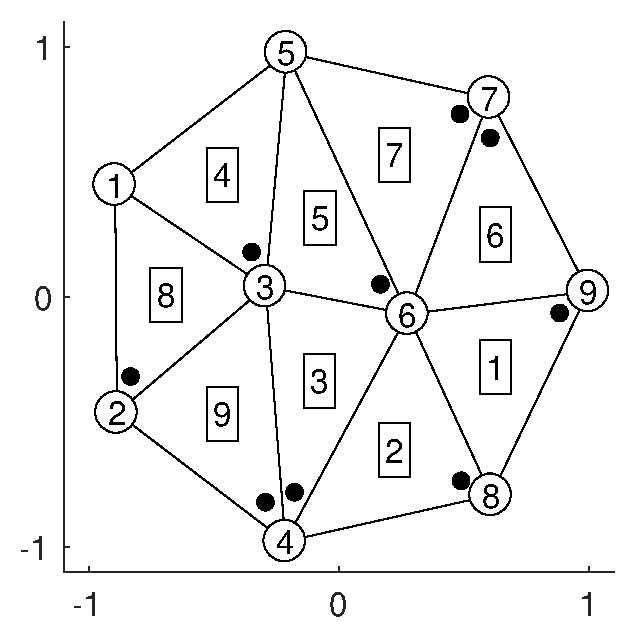
\includegraphics[width=0.4\textwidth]{fe_mesh_p1}
  }
  \caption{Triangulation.}
  \label{fig:fe_mesh_p1}
\end{figure}

While mathematically a triangulation is simply a collection of non-overlapping elements, we need a convenient means to represent the triangulation on a computer.  One approach is to store a table of \emph{node coordinates} and \emph{element-node connectivity}.  Tables~\ref{tb:fe_mesh_p1_coord} and \ref{tb:fe_mesh_p1_tri} are respectively the coordinate and connectivity tables associated with the triangulation shown in Figure~\ref{fig:fe_mesh_p1}. The connectivity table indicates that, for instance, element 7 is delineated by the nodes 7, 8, and 11; the coordinate table then indicates that the coordinates of these three nodes are $(0.33,0.66)$, $(0.43,0.31)$, and $(0.68,0.58)$, respectively.  Note that, in Figure~\ref{fig:fe_mesh_p1}, for each triangle, we indicate the first of the three nodes that delineate the triangle by a dot ($\bullet$); with this convention we have identical information presented in Figure~\ref{fig:fe_mesh_p1} in a visual form and Tables~\ref{tb:fe_mesh_p1_coord} and \ref{tb:fe_mesh_p1_tri} in an array form.

\begin{table}
  \centering
  \subfigure[coordinates]{
    \begin{tabular}{c|cc}
      node & $x_1$ & $x_2$ \\
      \hline
      $1$ & $0.00$ & $0.67$ \\ 
      $2$ & $0.00$ & $0.00$ \\ 
      $3$ & $0.00$ & $1.00$ \\ 
      $4$ & $0.00$ & $0.34$ \\ 
      $5$ & $0.32$ & $0.00$ \\ 
      $6$ & $0.33$ & $1.00$ \\ 
      $7$ & $0.33$ & $0.66$ \\ 
      $8$ & $0.43$ & $0.31$ \\ 
      $9$ & $0.66$ & $1.00$ \\ 
      $10$ & $0.68$ & $0.00$ \\ 
      $11$ & $0.68$ & $0.58$ \\ 
      $12$ & $1.00$ & $0.68$ \\ 
      $13$ & $1.00$ & $0.33$ \\ 
      $14$ & $1.00$ & $0.00$ \\ 
      $15$ & $1.00$ & $1.00$ \\  
    \end{tabular}
    \label{tb:fe_mesh_p1_coord}
  }
  \subfigure[connectivity]{
    \begin{tabular}{c|ccc}
      element & node 1 & node 2 & node 3 \\
      \hline
      $1$ & $8$ & $13$ & $11$ \\ 
      $2$ & $11$ & $13$ & $12$ \\ 
      $3$ & $15$ & $9$ & $12$ \\ 
      $4$ & $12$ & $9$ & $11$ \\ 
      $5$ & $2$ & $5$ & $4$ \\ 
      $6$ & $4$ & $5$ & $8$ \\ 
      $7$ & $7$ & $8$ & $11$ \\ 
      $8$ & $11$ & $9$ & $7$ \\ 
      $9$ & $1$ & $4$ & $7$ \\ 
      $10$ & $7$ & $4$ & $8$ \\ 
      $11$ & $8$ & $5$ & $10$ \\ 
      $12$ & $14$ & $13$ & $10$ \\ 
      $13$ & $13$ & $8$ & $10$ \\ 
      $14$ & $6$ & $7$ & $9$ \\ 
      $15$ & $6$ & $3$ & $1$ \\ 
      $16$ & $1$ & $7$ & $6$ \\ 
    \end{tabular}
    \label{tb:fe_mesh_p1_tri}
  }
  \caption{Node coordinate and connectivity table.}
  \label{tb:fe_mesh_p1}
\end{table}

The task of generating a triangulation for a given domain is called \emph{mesh generation} and a program that carries out the task is called a \emph{mesh generator} or \emph{meshers}.  Mesh generation is a non-trivial task.  In fact, the development of algorithms that can robustly and automatically generate high-quality triangulation for complex geometries in three dimensions is an area of ongoing research.  Nevertheless, because mesh generation is essential for any finite element discretization, there is a large number of commercial and open-source meshers.  Here we name a few user-friendly, open-source meshers. The \texttt{triangle} is a mesh generator developed by Richard Shewchuk which creates two-dimensional meshes with a guaranteed quality certificate (in terms of the minimum angle). The \texttt{tetgen} is a popular open-source three-dimensional mesher.  The \texttt{distmesh} is a \textsc{Matlab} mesh generator developed by Per-Olof Persson, which is particularly user friendly.  The mesh shown in Figure~\ref{fig:fe_Mesh_p1} was in fact generated by \texttt{distmesh}.  We will extensively use \texttt{distmesh} to generate meshes in this course due to its ease of use.

\section{Linear Lagrange finite element space}
\label{sec:fe_lin_tri}
We now consider the construction of a piecewise linear polynomial space associated with the triangulation $\calT_h$. We recall that our variational (or weak) formulation requires that the finite element space is a subset of the function space for the exact PDE, which, for second-order elliptic equations, is some $\calV$ which is a subset of $H^1(\Omega)$. Since our finite element space $\calV_h$ is piecewise polynomial, the continuity across element boundaries is the necessary and sufficient condition for $\calV_h \subset \calV$.  Hence, our goal is to devise a systematic procedure to represent any functions in
\begin{equation}
  \calV_h \equiv \{ v \in C^0(\overline \Omega) \ | \ v|_K \in \PP^1(K), \ K \in \calT_h \},
  \label{eq:fe_lin_Vh}
\end{equation}
where $C^0(\overline \Omega)$ is the space of continuous functions over $\overline \Omega$.  Figure~\ref{fig:fe_fun_p1} shows an example of a continuous, piecewise-linear function in $\calV_h$ associated with $\calT_h$ shown in Figure~\ref{fig:fe_mesh_p1}.
\begin{figure}
  \centering
  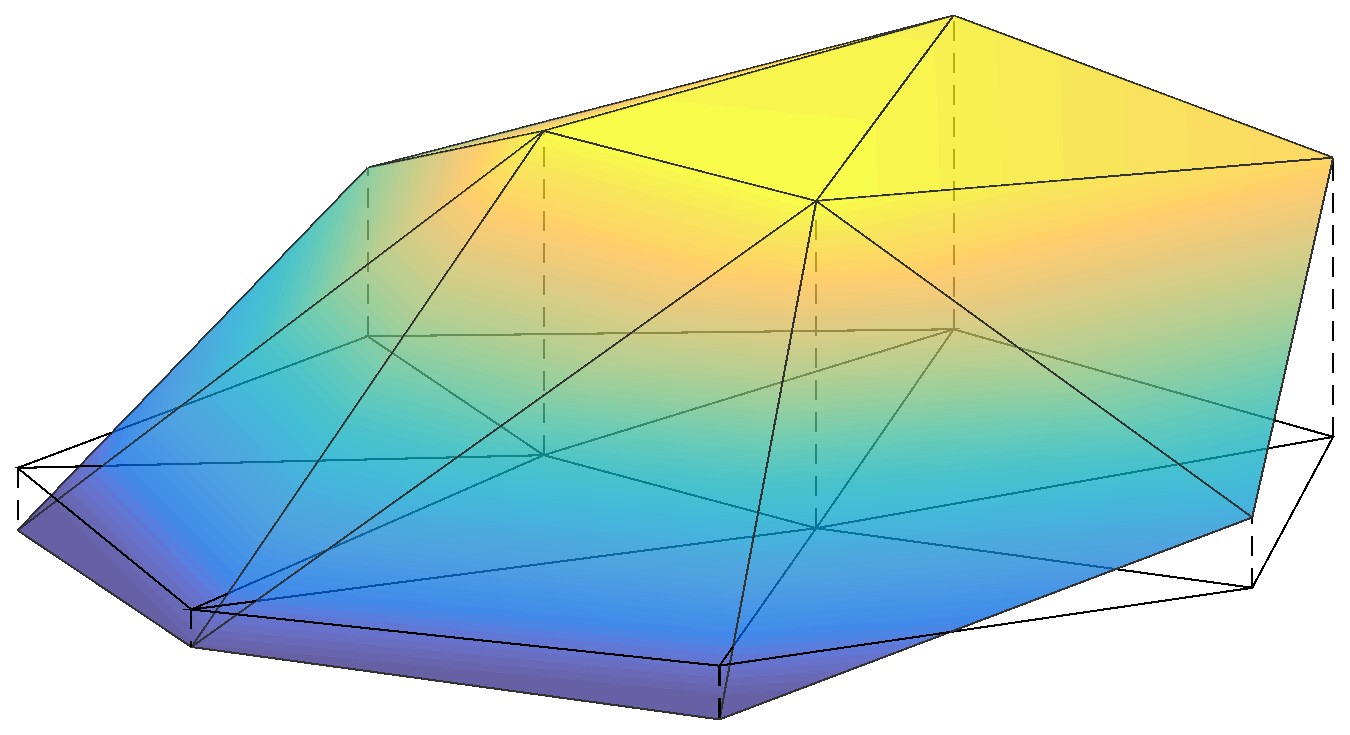
\includegraphics[width=0.45\textwidth]{fe_fun_p1}
  \caption{A function in a linear finite element space.}
  \label{fig:fe_fun_p1}
\end{figure}

We now need a convenient means to describe functions in $\calV_h$ given by~\eqref{eq:fe_lin_Vh}, such as the one shown in Figure~\ref{fig:fe_fun_p1}.  Specifically, we need to pick \emph{global degrees of freedom} with which we can uniquely describe any function in $\calV_h$.  While the choice of global degrees of freedom is not unique, one convenient choice is the value of the function at the nodes of the triangulation~$\calT_h$.  For instance, the piecewise linear function shown in Figure~\ref{fig:fe_fun_p1} can be described uniquely by the values that the function takes at 16 nodes of the triangulation~$\calT_h$ shown in Figure~\ref{fig:fe_mesh_p1}.  This may be intuitively obvious, 



Our approach to construct the piecewise polynomial space is to first define a polynomial space on a \emph{reference element} (or a \emph{canonical element}) and then to map the polynomial functions to the actual elements that comprise the triangulation.  As such, we first introduce the \emph{reference triangle} $\tilde K$.  While the definition of a reference triangle is not universal, our reference triangle is shown in Figure~\ref{fig:fe_ref_tri}.  The triangle is a right triangle delineated by three vertices
\begin{equation*}
  v^1 \equiv (0,0), \quad v^2 \equiv (1,0), \quad \text{and} \quad v^3 \equiv (0,1).
\end{equation*}
The vertices are ordered in the counter-clockwise manner. We also denote the three edges of the triangles by
\begin{equation*}
  e^1 \equiv (v^2,v^3), \quad e^2 \equiv (v^3,v^1), \quad \text{and} \quad e^3 \equiv (v^1,v^2).
\end{equation*}
We choose the convention that the edge number is the same as the vertex number of the vertex on the other side of the triangle. Each edge is oriented such that the collection of the three edges defines the triangle in the counter-clock orientation.  

\begin{figure}
  \centering
  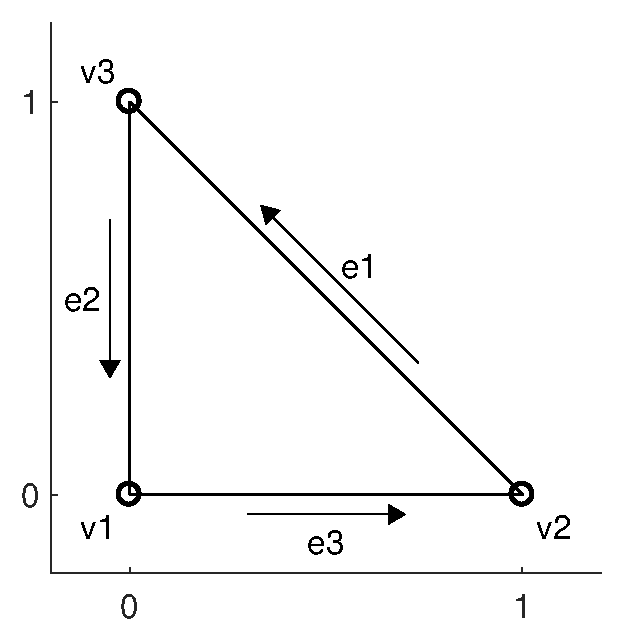
\includegraphics[width=0.3\textwidth]{ref_tri}
  \caption{Reference triangle.}
  \label{fig:fe_ref_tri}
\end{figure}

Having introduced the reference triangle, we now introduce arguably the simplest finite element in two dimensions: linear Lagrange element on the reference triangle. A linear function in $\PP^1(\tilde K)$ takes on the form $a_1 + a_2 \tilde x_1 + a_3 \tilde x_2$ and has three degrees of freedom; we hence need to identify a linear independent set of three linear functions.  In our case, we wish to identify a set of three linear \emph{Lagrange basis functions} for the space.  To this end, we choose for our Lagrange interpolation nodes the three vertices of the triangle
\begin{equation*}
  \tilde x^{(1)} = (0,0), \quad \tilde x^{(2)} = (1,0), \quad \text{and} \quad \tilde x^{(3)} = (0,1),
\end{equation*}
as shown in Figure~\ref{fig:fe_ref_tri_p1}. Our goal is to find the Lagrange basis functions
\begin{equation*}
  \{ \tilde \phi_1, \tilde \phi_2, \tilde \phi_3 \}
\end{equation*}
that lie in the $\PP^1(\tilde K)$ space and satisfy the interpolation condition
\begin{equation}
  \tilde \phi_i(\tilde x^{(j)}) = \delta_{ij} \quad i,j = 1,\dots,3.
% \equiv
% \begin{cases}
%   1, \quad i = j \\
%%   0, \quad i \neq j
% \end{cases};
   \label{eq:fe_interp_tri}
\end{equation}
Here, $\delta_{ij}$ denotes the \emph{Kronecker delta} such that $\delta_{ij} = 1$ for $i = j$ and $\delta_{ij} = 0$ for $i \neq j$.

\begin{figure}
  \centering
  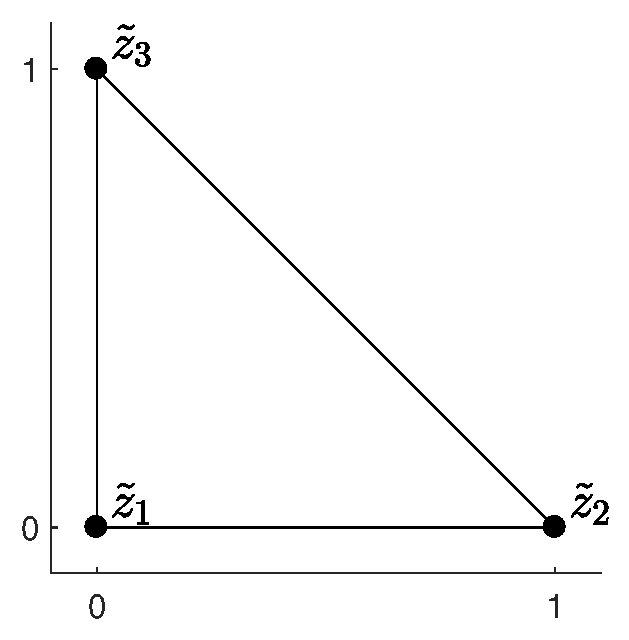
\includegraphics[width=0.3\textwidth]{ref_tri_p1}
  \caption{Linear Lagrange finite element on the reference triangle.}
  \label{fig:fe_ref_tri_p1}
\end{figure}


    While we may identify the Lagrange basis functions for the linear space by inspection, we here follow a more systematic procedure that apply to more complex domains and higher-order polynomials.  To this end, we first note that any linear function can be expressed as a linear combination of a monomial basis
\begin{equation*}
  \{ 1, \tilde x_1, \tilde x_2\}.
\end{equation*}
Since linear Lagrange basis functions are also linear functions, we can express the basis functions in terms of the monomial basis:
\begin{equation}
  \tilde \phi_j(\tilde x) = a^{(j)}_1 + a^{(j)}_2 \tilde x_1 + a_3^{(j)} \tilde x_2 \quad j = 1, 2, 3.
  \label{eq:fe_lin_tri_rep}
\end{equation}
We now apply the interpolation condition~\eqref{eq:fe_interp_tri} to find the coefficients.  For instance, $\tilde \phi_1$ must satisfy
\begin{equation*}
  \bmat{ccc}
  1 & \tilde x_1^{(1)} & \tilde x_2^{(1)} \\
  1 & \tilde x_1^{(2)} & \tilde x_2^{(2)} \\
  1 & \tilde x_1^{(3)} & \tilde x_2^{(3)} \\
  \emat
  \bmat{ccc}
  a_1^{(1)} \\ a_2^{(1)} \\ a_3^{(1)}
  \emat
  =
  \bmat{ccc}
  1 \\ 0 \\ 0.
  \emat
\end{equation*}
We can also pose a single matrix equation for the monomial coefficients of all three shape functions: 
\begin{equation*}
  \underbrace{ \bmat{ccc}
      1 & \tilde x_1^{(1)} & \tilde x_2^{(1)} \\
  1 & \tilde x_1^{(2)} & \tilde x_2^{(2)} \\
  1 & \tilde x_1^{(3)} & \tilde x_2^{(3)} \\
  \emat }_{\equiv V}
  \underbrace{ 
  \bmat{ccc}
  a_1^{(1)} & a_1^{(2)} & a_1^{(3)} \\
  a_2^{(1)} & a_2^{(2)} & a_2^{(3)} \\
  a_3^{(1)} & a_3^{(2)} & a_3^{(3)} \\
  \emat
  }_{\equiv A}
  =
  \bmat{ccc}
  1 & 0 & 0 \\
  0 & 1 & 0 \\
  0 & 0 & 1
  \emat.
\end{equation*}
We note that the matrix $V$ in the left hand side is the \emph{Vandermonde matrix} associated with our monomial basis evaluated at the Lagrange interpolation points $\{\tilde x^{(1)},\tilde x^{(2)}, \tilde x^{(3)}\}$.  The matrix $V$ is non-singular as long as the interpolation points are not collinear, which is equivalent to the condition that the triangle have a finite area; the condition is obviously satisfied for our reference triangle $\tilde K$.  For completeness, we provide the explicit expression for the coefficient $A$
\begin{equation*}
  A = \bmat{ccc}
  1 & 0 & 0\\
  -1 & 1 & 0 \\
  -1 & 0 & 1
  \emat,
\end{equation*}
the explicit expressions for the basis functions
\begin{align}
  \tilde \phi_1(\tilde x) &= 1 - \tilde x_1 - \tilde x_2 \notag \\
  \tilde \phi_2(\tilde x) &= \tilde x_1 \label{eq:fe_lin_tri_expl} \\
  \tilde \phi_3(\tilde x) &= \tilde x_2, \notag
\end{align}
and in Figure~\ref{fig:fe_shape_tri_p1} visual representation of the basis functions.

\begin{figure}
  \centering
  \subfigure[$\tilde \phi_1$]{
    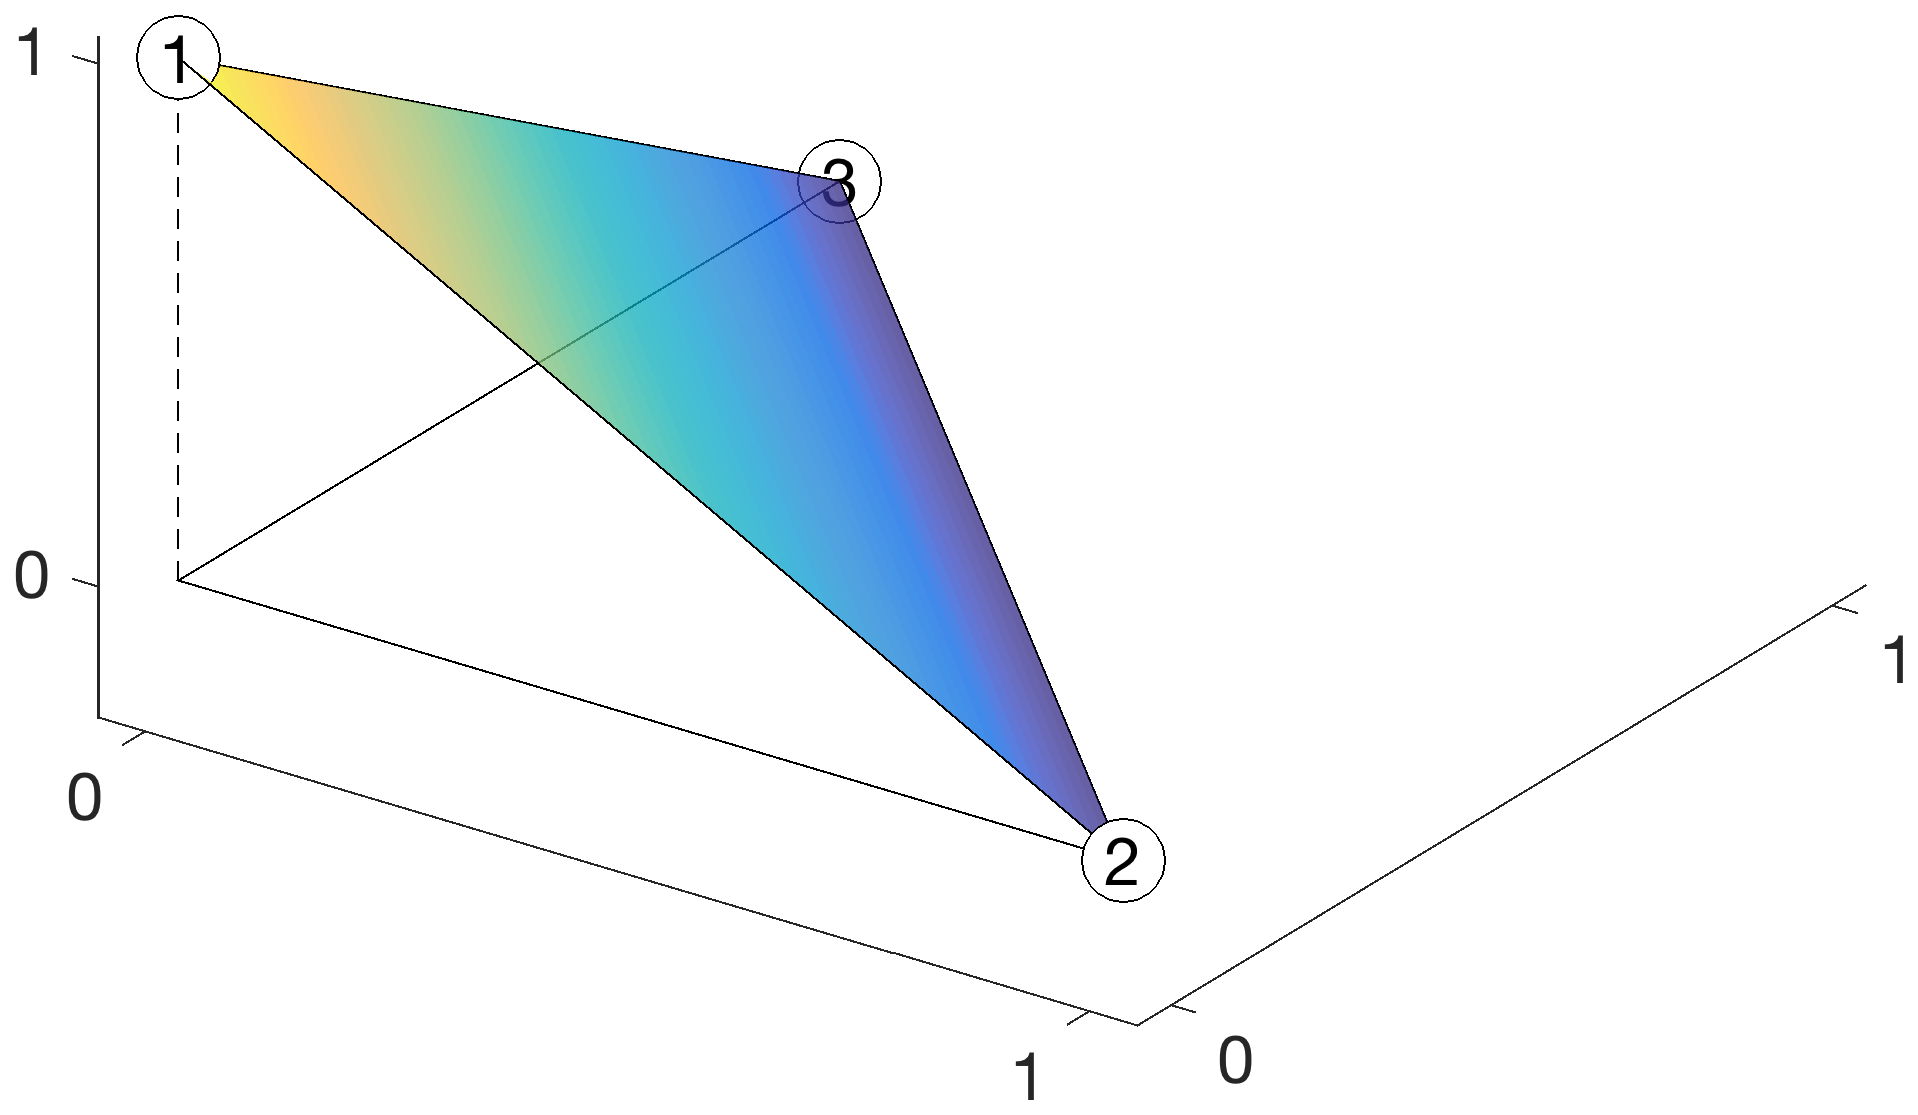
\includegraphics[width=0.3\textwidth]{shape_tri_p1_1}
  }
  \subfigure[$\tilde \phi_2$]{
    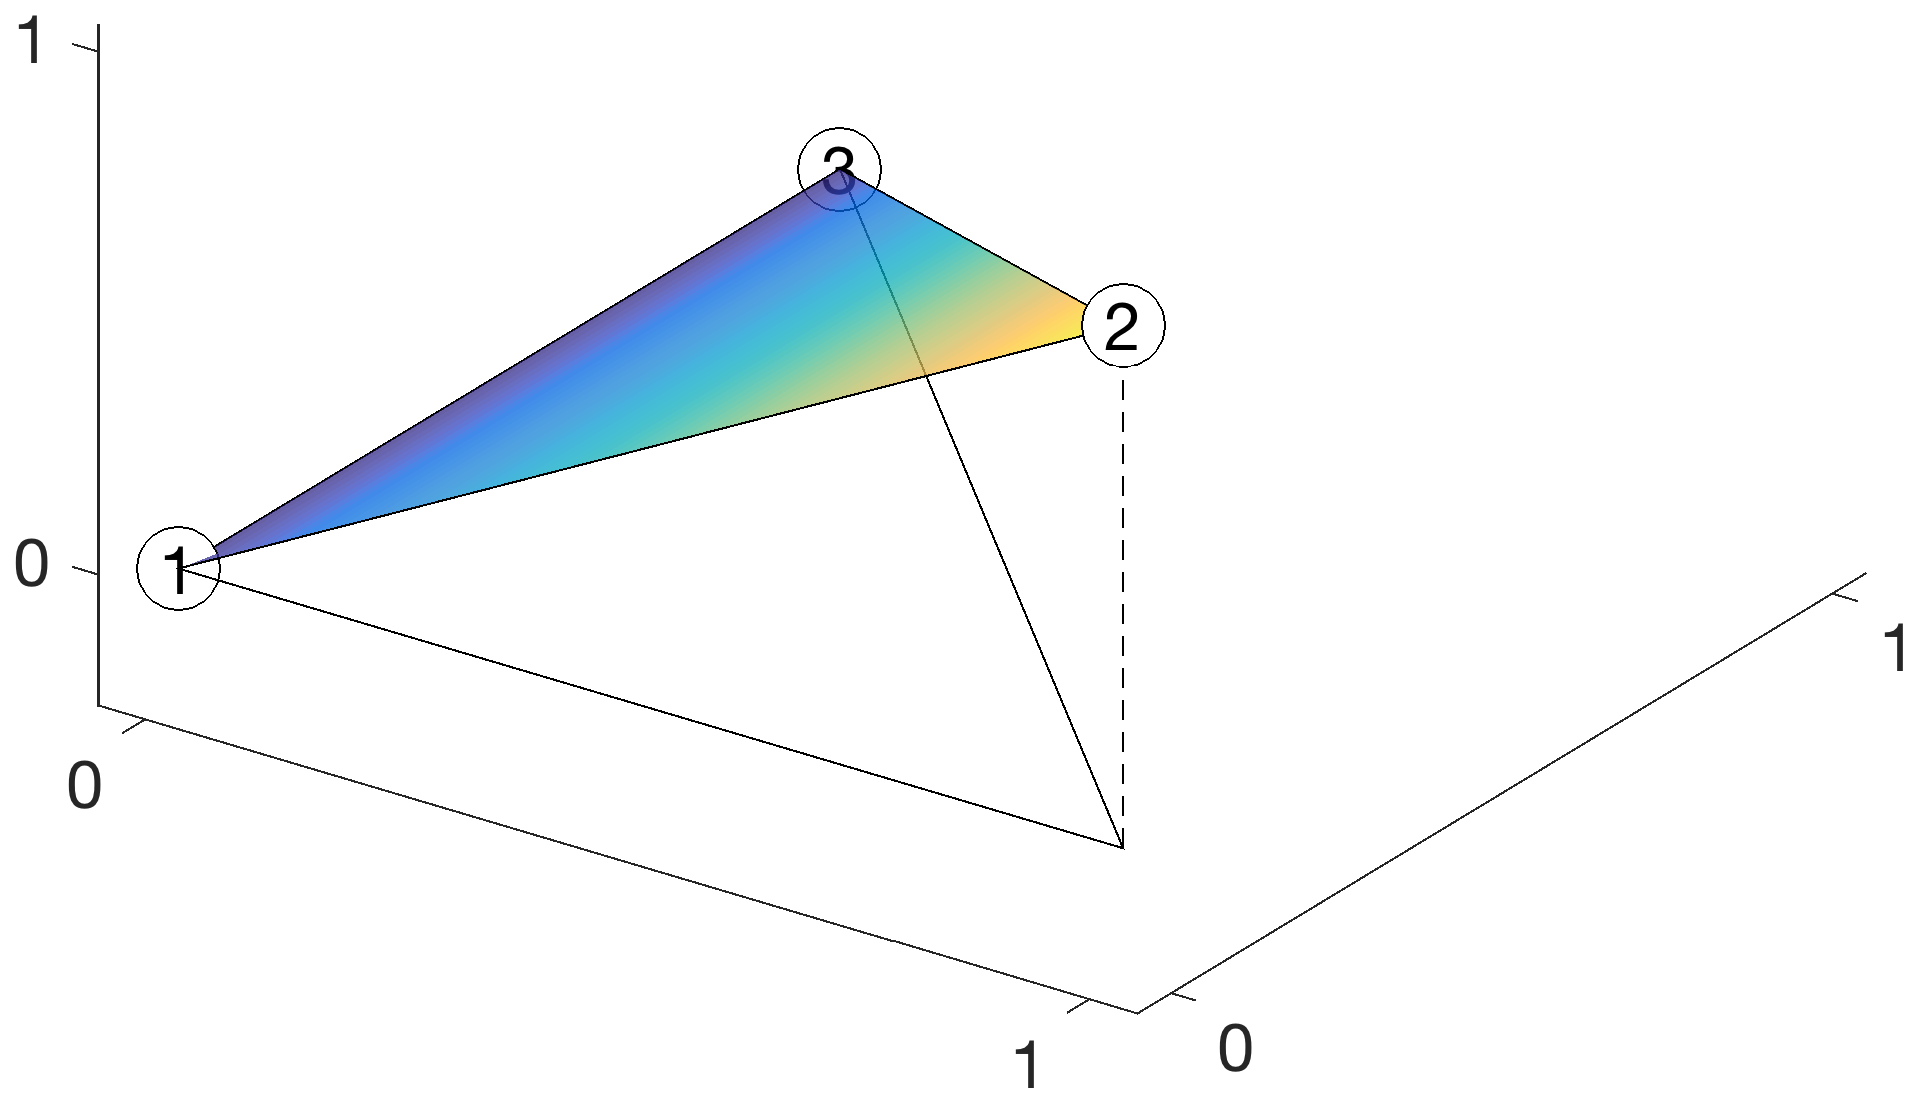
\includegraphics[width=0.3\textwidth]{shape_tri_p1_2}
  }
  \subfigure[$\tilde \phi_3$]{
    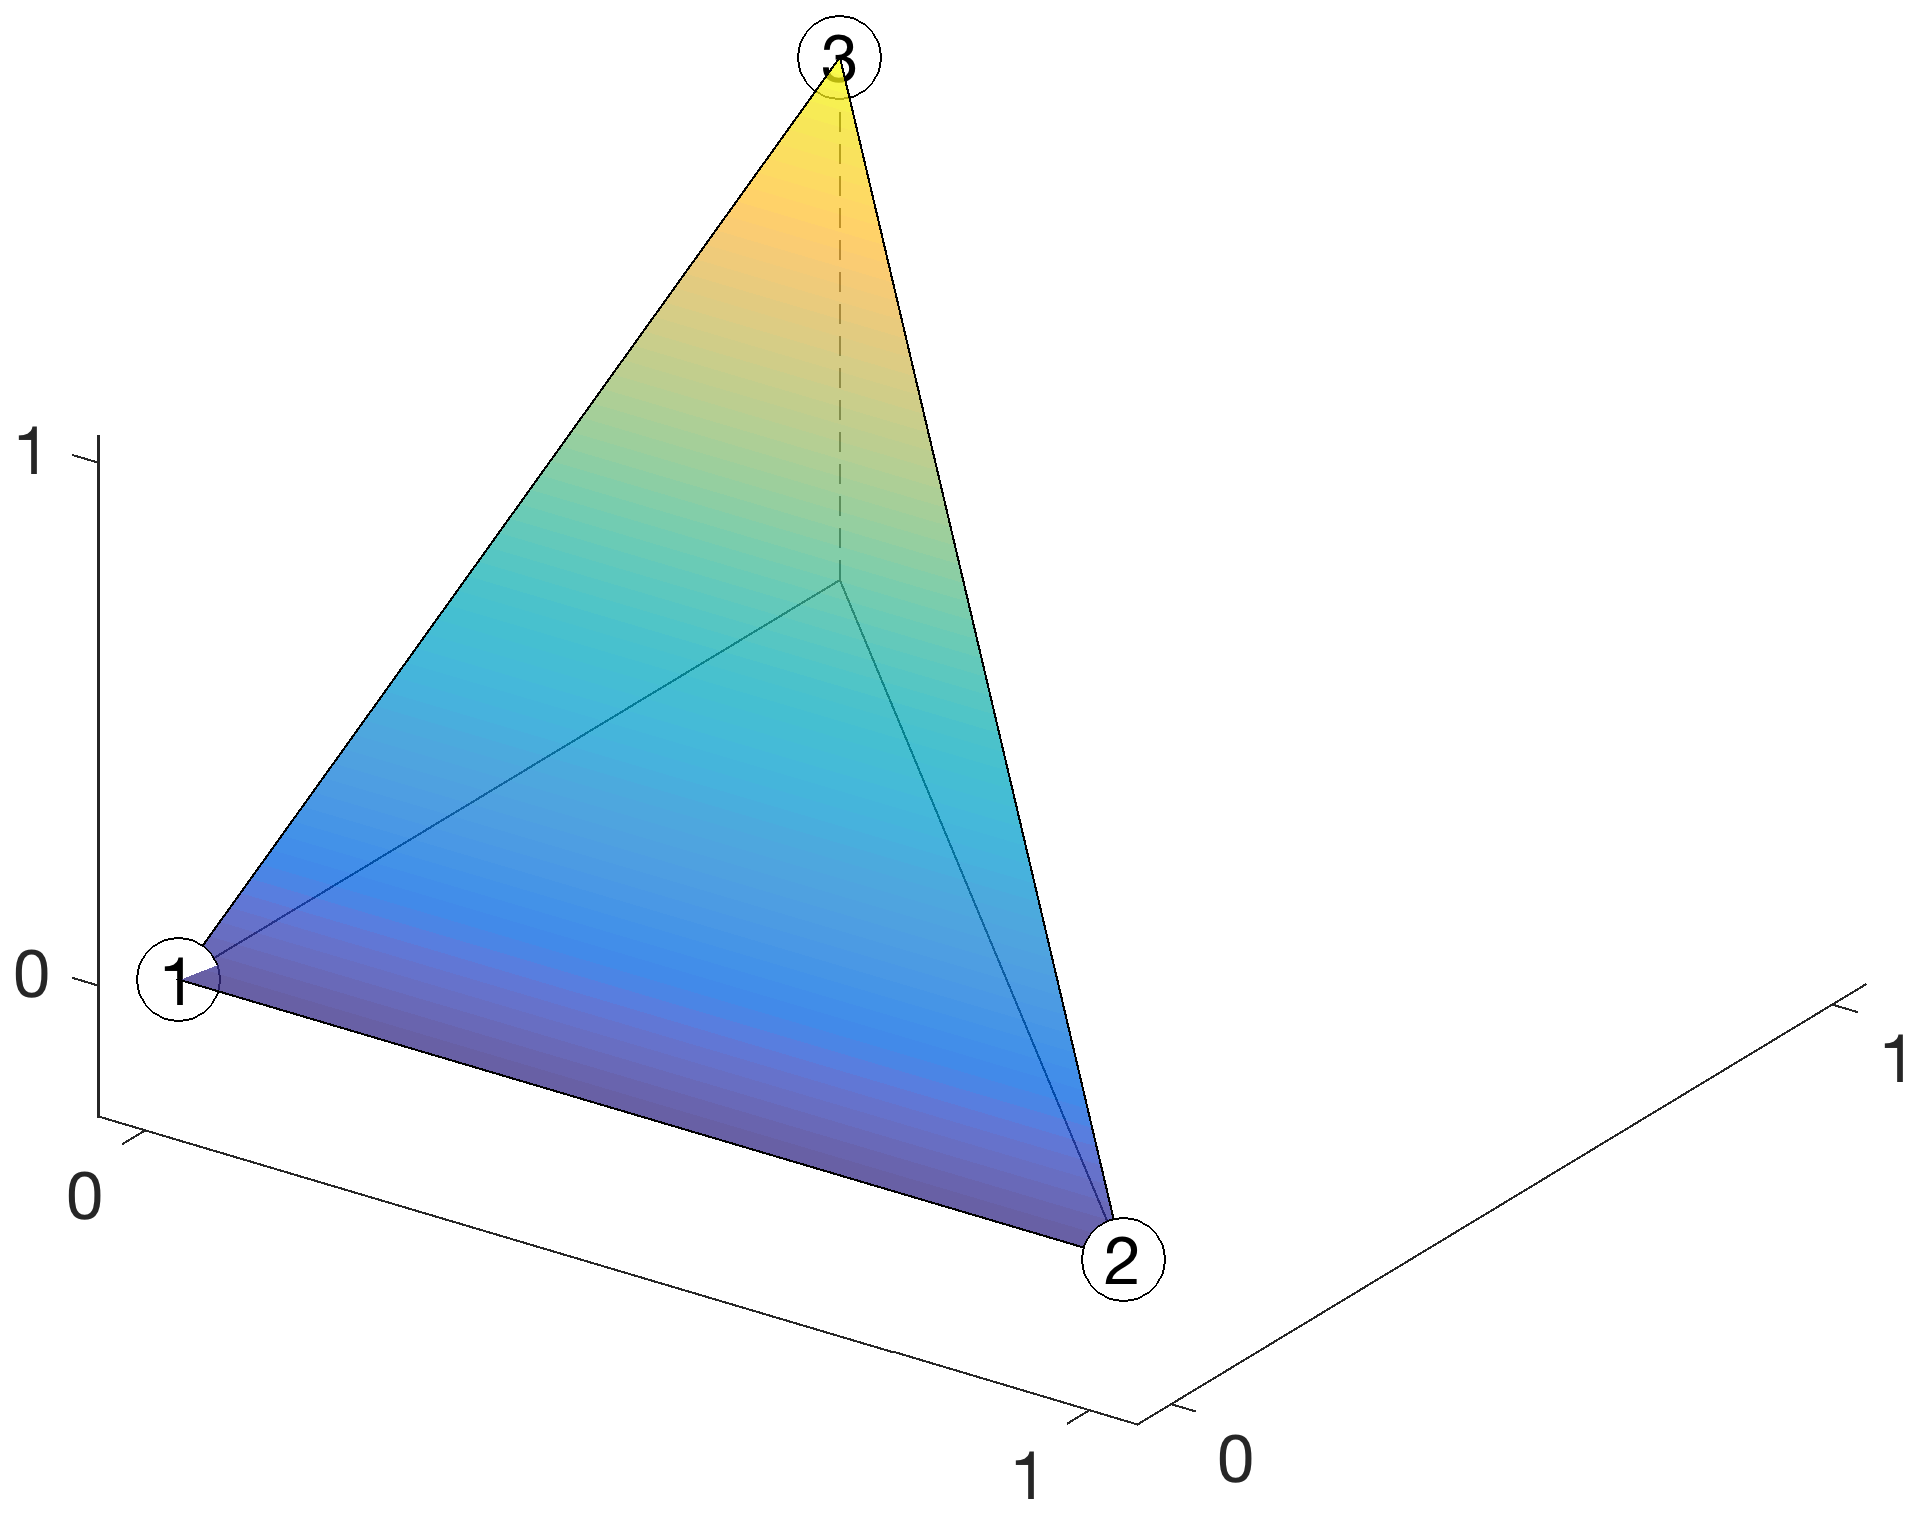
\includegraphics[width=0.3\textwidth]{shape_tri_p1_3}
  }
  \caption{Linear Lagrange shape functions on the reference triangle.}
  \label{fig:fe_shape_tri_p1}
\end{figure}

Once we find the coefficients of the shape functions, we can evaluate the value of the functions at any point in the triangle by evaluating~\eqref{eq:fe_lin_tri_rep}. We can also differentiate~\eqref{eq:fe_lin_tri_rep} to obtain the gradient of the shape functions:
\begin{align*}
  \pp{\tilde \phi_j}{\tilde x_1}(x) = a_2^{(j)}
  \quad \text{and} \quad
  \pp{\tilde \phi_j}{\tilde x_2}(x) = a_3^{(j)}, \quad j = 1,2,3.
\end{align*}
For the linear Lagrange element, the derivatives are constant over the element because the shape functions are linear.

Using the linear Lagrange basis functions, we can now represent any function $v$ that is in $\PP^1(\tilde K)$.  Specifically, we may represent $v \in \PP^1(\tilde K)$ in terms of a coefficient vector $\hat v \in \RR^3$ as
\begin{equation*}
  v(\tilde x) = \sum_{j=1}^{3} \hat v_j  \tilde \phi_j(\tilde x) \quad \forall \tilde x \in \tilde K
\end{equation*}
for $\hat v_j \equiv v(\tilde x^j)$, $j = 1,2,3$.  We hence have a one-to-one mapping between \emph{any} element in $\PP^1(\tilde K)$ and the associated coefficient vector in $\RR^3$.  For the linear Lagrange basis functions, the coefficients $\hat v \in \RR^3$ is associated with the values of the function at the vertices of the triangle.

Before we introduce other finite elements, we use the linear Lagrange element as an example to describe three properties that formally defines a \emph{finite element}:
\begin{enumerate}
\item the domain $\tilde K$ over which the element is defined; e.g., the reference triangle $\tilde K$ defined by vertices shown in Figure~\ref{fig:fe_ref_tri}.
\item the finite-dimensional linear space of functions; e.g., the linear polynomial space $\PP^1(\tilde K)$ spanned by $\{ 1, \tilde x_1, \tilde x_2 \}$.
\item the degree of freedom used to describe functions; e.g., the values of the function at the vertices of the triangle.
\end{enumerate}

\section{Isoparametric mapping}
In Section~\ref{sec:fe_lin_tri}, we introduced a linear finite element associated with a reference triangle.  We now wish to map the finite element to the physical elements that constitute the triangulation $\calT_h$.  To this end, we introduce the procedure based on \emph{isoparametric mapping}.

\begin{figure}
  \centering
  \subfigure[reference element]{
    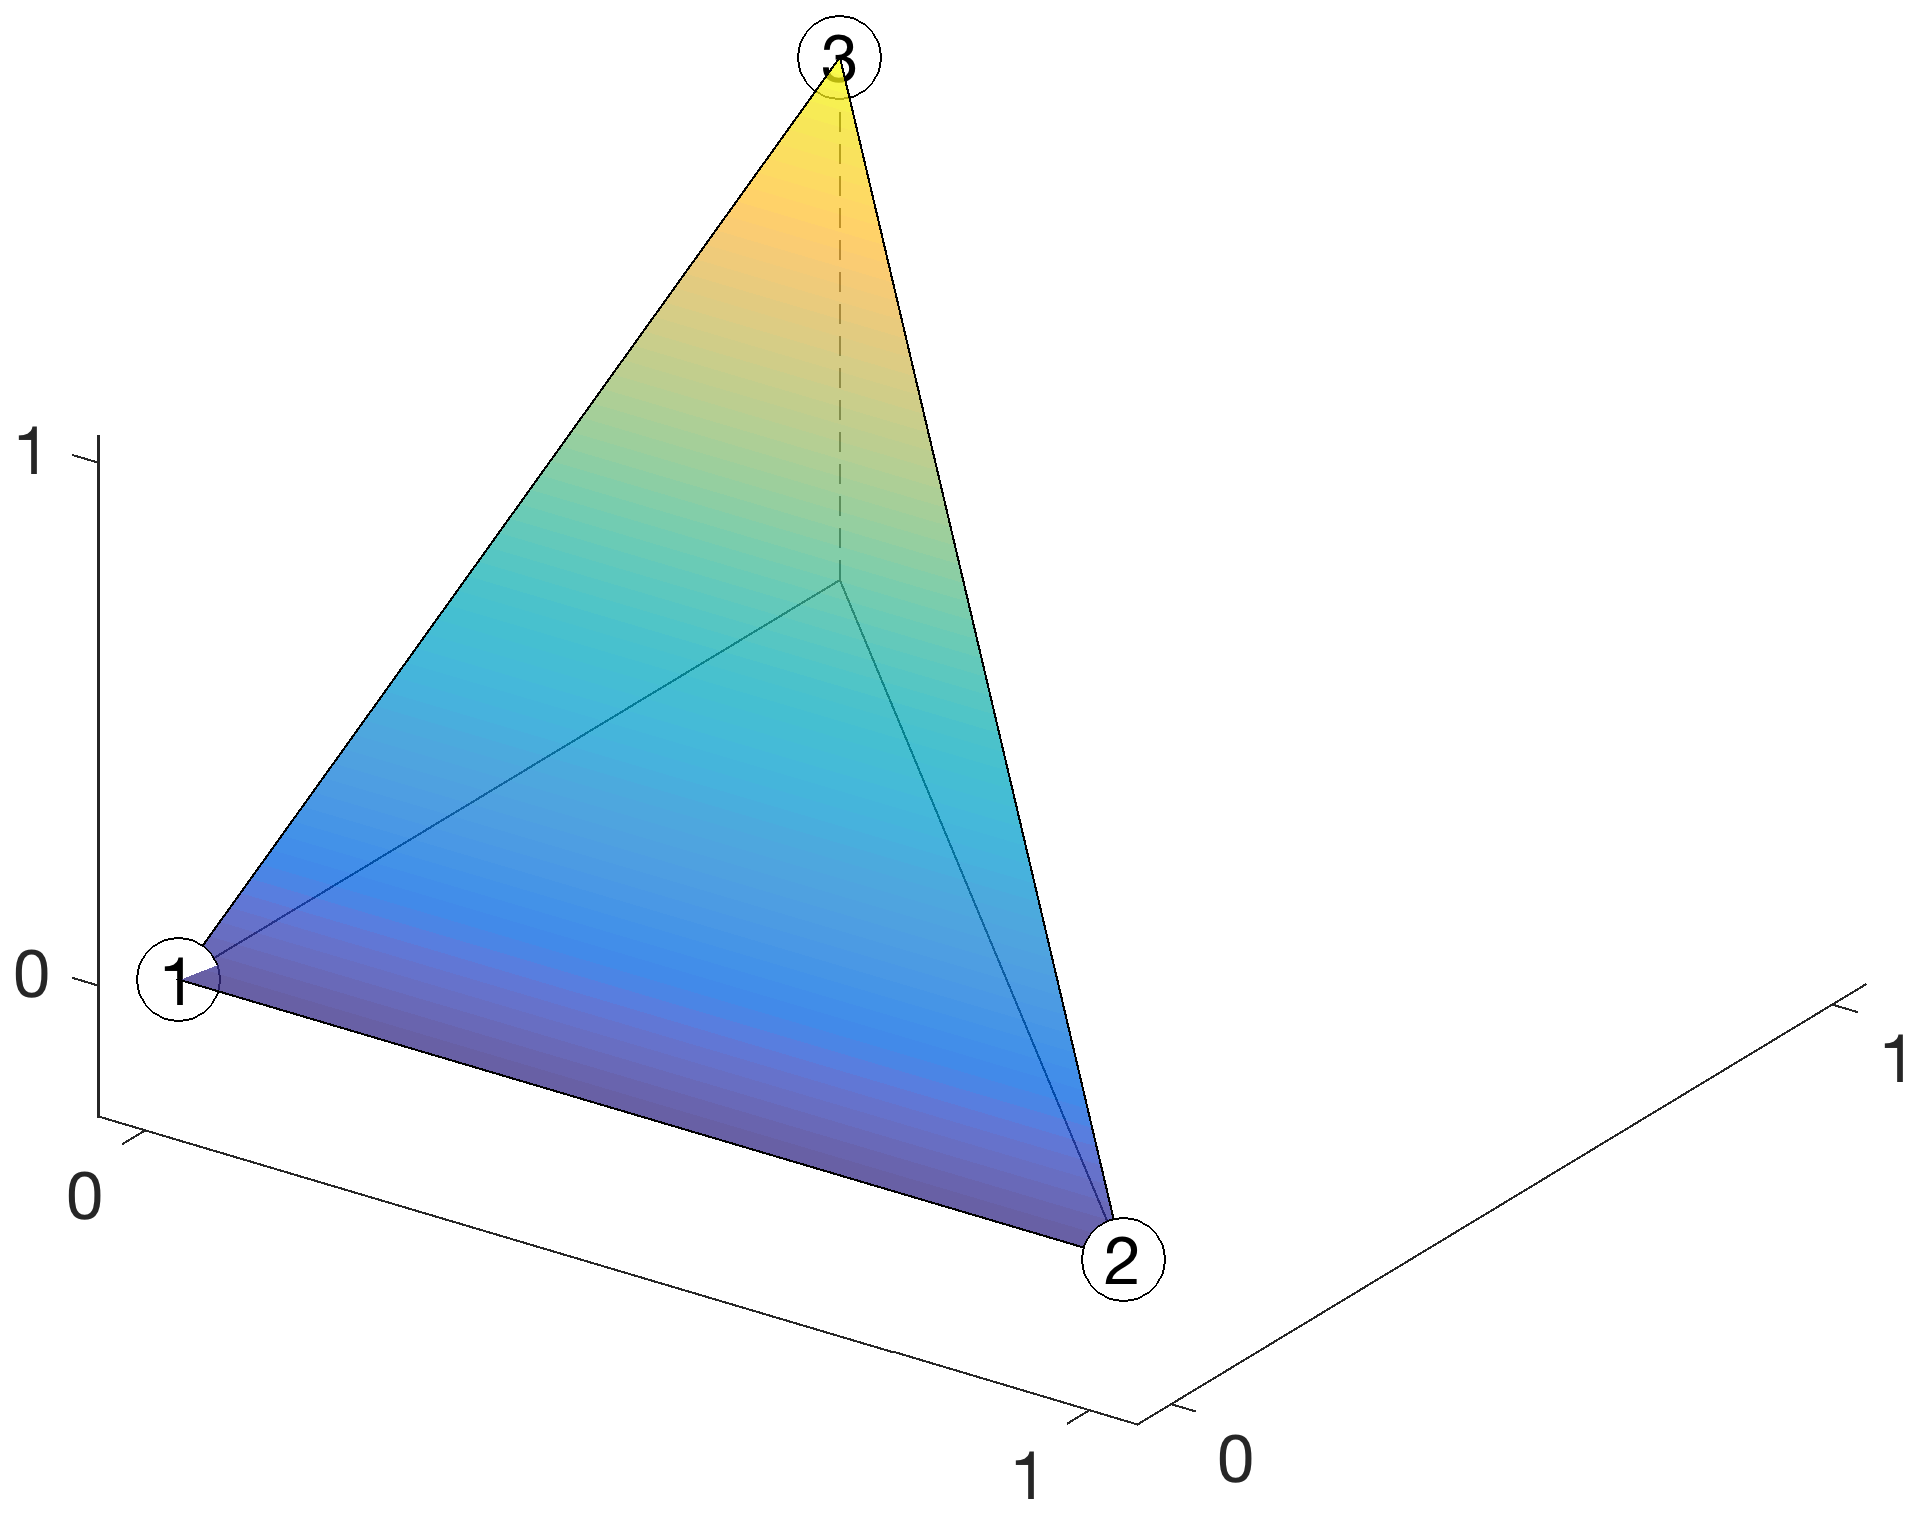
\includegraphics[width=0.3\textwidth]{shape_tri_p1_3}
  }
  \subfigure[physical element]{
    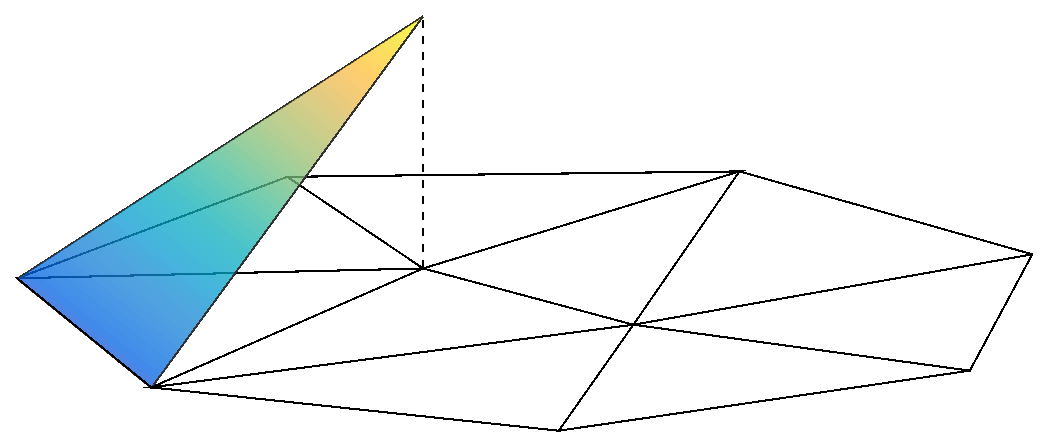
\includegraphics[width=0.4\textwidth]{shape_global_p1_part}
  }
\end{figure}

The isoparametric mapping is a mapping from the reference element to the physical element such that (i) the mapping is polynomial and (ii) the Lagrange interpolation points of the reference element are mapped to the respective Lagrange interpolation points of the physical element. For instance, for a linear triangle, the mapping is linear and vertices of the reference triangle are mapped to the respective vertices of the physical triangle.   Algebraically, the isoparametric mapping that maps $\xi \in \tilde K$ to $x \in K$ is given by
\begin{equation}
  x_i(\xi) = \sum_{j=1}^{n_s} x^j_i \tilde \phi_j(\xi), \quad i = 1,\dots,d,
  \label{eq:fe_iso_map}
\end{equation}
where $x_i^j$ is the $i$-th coordinate of the $j$-th interpolation point, and $\tilde \phi_i$ is the Lagrange basis function on the reference element associated with the $i$-th interpolation node, and $n_s$ is the number of basis functions, which is equal to the number of interpolation points.
As a concrete example, consider the triangulation shown in Figure~\ref{fig:fe_mesh_p1} (and encoded in Table~\ref{tb:fe_mesh_p1}).  For the physical element 7, we have
\begin{equation*}
  x^1 = v^7 = (0.33,0.66), \quad 
  x^2 = v^8 = (0.43,0.31), \quad \text{and} \quad
  x^3 = v^{11} = (0.68,0.58);
\end{equation*}
the associated basis functions are given by~\eqref{eq:fe_lin_tri_expl}.
The map~\eqref{eq:fe_iso_map} satisfies the two conditions of isoparametric mapping:
\begin{itemize}
\item[(i)] Because the Lagrange basis functions are polynomial, the mapping $\xi \mapsto x$ is polynomial.
\item[(ii)] The $k$-th interpolation point of the reference triangle $\xi^k$ is mapped to the $k$-th interpolation point of the physical triangle $x^k$ since $x(\xi^k) = \sum_{j=1}^{n_s} x^j \tilde \phi_j(\xi^k) = \sum_{j=1}^{n_s} x^j \delta_{jk} = x^k$.
\end{itemize}
Hence, $\tilde K \ni \xi \mapsto x \in K$ is an isoparametric mapping.

With this mapping, we can now construct 

\begin{figure}
  \centering
  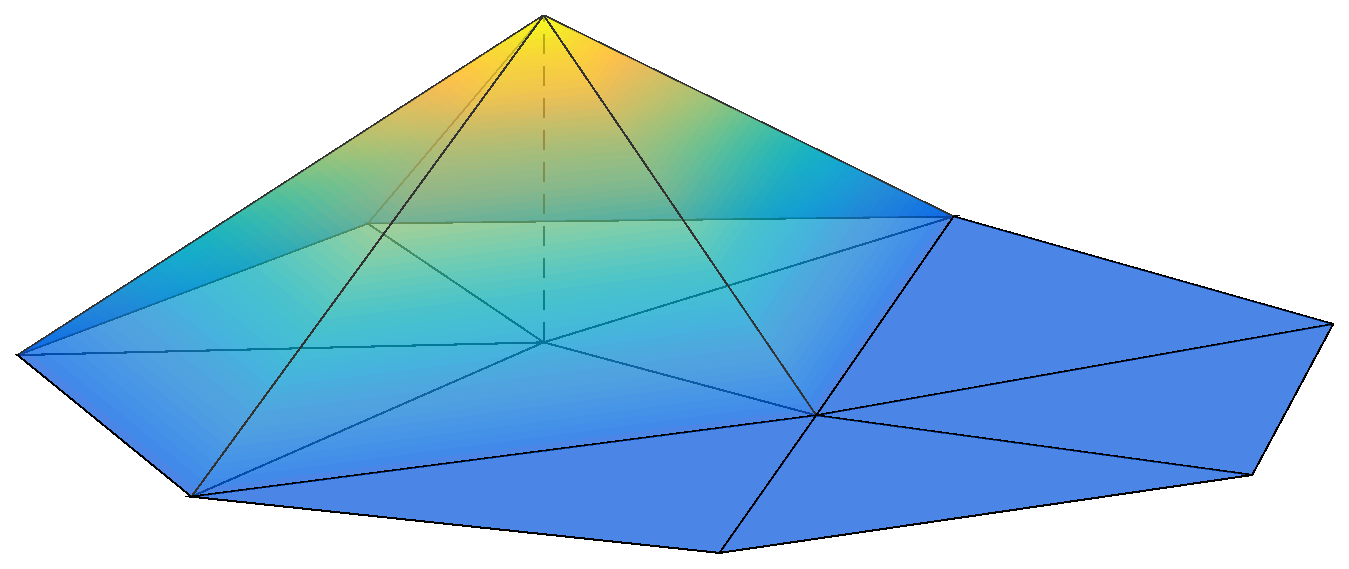
\includegraphics[width=0.48\textwidth]{shape_global_p1}
\end{figure}


We can differentiate~\eqref{eq:fe_iso_map} to evaluate the \emph{Jacobian} of the isoparametric mapping; the $(i,j)$ entry of the Jacobian $J \equiv \pp{x}{\xi_j} \in \RR^{d \times d}$, is given by
\begin{equation*}
  J_{ij} = \pp{x_i}{\tilde x_j} = \sum_{j=1}^{n_s} x^j_i \pp{\tilde \phi_i}{\tilde x_j} .
\end{equation*}

\begin{equation*}
  dx = \text{det}(J) d\tilde x
\end{equation*}

\begin{equation*}
  \pp{\xi}{x} = \left( \pp{x}{\xi} \right)^{-1}
\end{equation*}

\begin{equation*}
  \phi(x) = \tilde \phi (\xi)
\end{equation*}

\begin{equation*}
  \pp{\phi}{x_i}(x) = \left. \pp{\tilde \phi}{\xi_j} \right|_\xi  \left. \pp{\xi_j}{x_i} \right|_\xi
\end{equation*}



For a quadratic triangle, the mapping is quadratic and vertices and mid-edge nodes of the reference triangle are mapped to the respective vertices and mid-edge nodes of the physical triangle.

Formally, a finite element space is parametrized by the following three properties:
\begin{enumerate}
\item the triangulation $\calT_h$ of $\Omega$;
\item the type of functions that constitutes the space (e.g., piecewise linear polynomial);
\item the degrees of freedom used to describe functions in the space.
\end{enumerate}
The first two are apparent from the definition of the finite element space~\eqref{eq:fe_space}.  The last property determines how a function $v \in \calV_h$ is represented on a computer.  Specifically, given a $N$-dimensional function space $\calV_h$, we assign $N$ degrees of --- by choosing $N$ basis functions --- such that the a function $v \in \calV_h$ can be uniquely described by $N$ real numbers.  We will clarify this third property in Section~\ref{sec:fe_map}.

\section{Quadratic Lagrange finite element on a triangle}
We now introduce a quadratic Lagrange finite element on a triangle. A quadratic function in $\PP^2(\tilde K)$ takes on the form $a_1 + a_2 \tilde x_1 + a_3 \tilde x_2 + a_4 \tilde x_1^2 + a_5 \tilde x_1 \tilde x_2 + a_6 \tilde x_2^2$ and ahs six degrees of freedom; we hence wish to identify a linearly independently set of six quadratic Lagrange basis functions.  To this end, we choose for our Lagrange interpolation nodes the three vertices of the triangle and three points at the middle of the edges
\begin{equation*}
  x^{(1)} = (0,0), \quad x^{(2)} = (1,0), \quad x^{(3)} = (0,1), \quad x^{(4)} = (1/2,1/2), \quad x^{(5)} = (0,1/2), \quad x^{(6)} = (1/2,0),
\end{equation*}
as shown in Figure~\ref{fig:fe_ref_tri_p2}.  The ordering of the quadratic nodes is not universal in the finite element literature; we here adhere the convention that, for $i \in \{4,5,6\}$, the $i$-th node is on the midpoint of the $i-3$-th edge of the reference triangle. Our goal is to find the Lagrange basis functions $\{\tilde \phi_i\}_{i=1}^6$ that lie in the $\PP^2(\tilde K)$ space and satisfy the interpolation condition $\tilde \phi_i(\tilde x^{(j)}) = \delta_{ij}$.

\begin{figure}
  \centering
  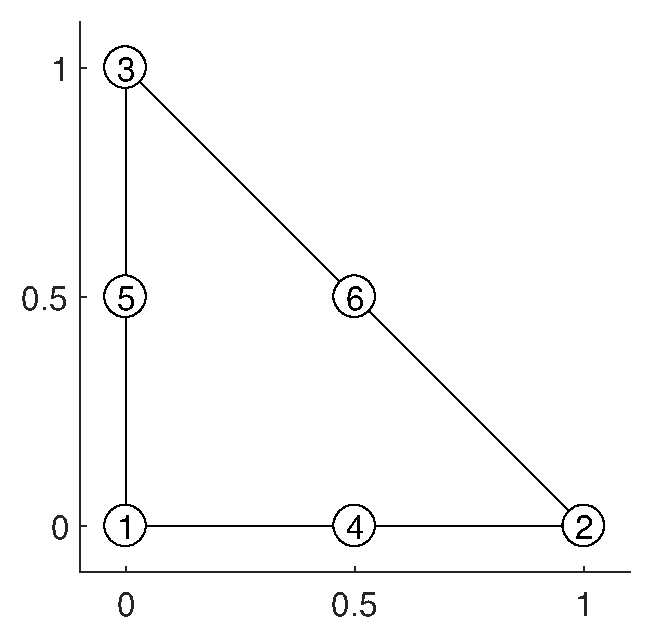
\includegraphics[width=0.3\textwidth]{ref_tri_p2}
  \caption{Quadratic Lagrange finite element on the reference triangle.}
  \label{fig:fe_ref_tri_p2}
\end{figure}


We now employ the procedure used in Section~\ref{sec:fe_lin_tri} to generate the quadratic Lagrange basis. We first express the basis functions in terms of the monomial basis
\begin{equation}
  \tilde \phi_j(\tilde x) = a_1^{(j)} + a_2^{(j)} \tilde x_1 + a_3^{(j)} \tilde x_2 + a_4^{(j)} \tilde x_1^2 + a_5^{(j)} \tilde x_1 \tilde x_2 + a_6^{(j)} \tilde x_2^2 \quad j = 1,\dots,6;
  \label{eq:fe_quad_tri_rep}
\end{equation}
we then express the interpolation condition $\tilde \phi_i(\tilde x^{(j)}) = \delta_{ij}$ as a $6 \times 6$ matrix system
\begin{equation*}
  V A = I,
\end{equation*}
where $A_{ij} = a^{(j)}_i$, $i,j = 1,\dots,6$, and the $i$-th row of the Vandermonde matrix $V \in \RR^{6 \times 6}$ is
\begin{equation*}
  V_{i:} = \bmat{cccccc} 1 & \tilde x^{(i)}_1 & \tilde x^{(i)}_2 &  (\tilde x^{(i)}_1)^2 & \tilde x^{(i)}_1 \tilde x^{(i)}_2 & (\tilde x^{(i)}_2)^2 \emat .
\end{equation*}
The linear system has a unique solution.  Figure~\ref{fig:fe_shape_tri_p2} shows the six basis functions.

\begin{figure}
  \centering
  \subfigure[$\tilde \phi_1$]{
    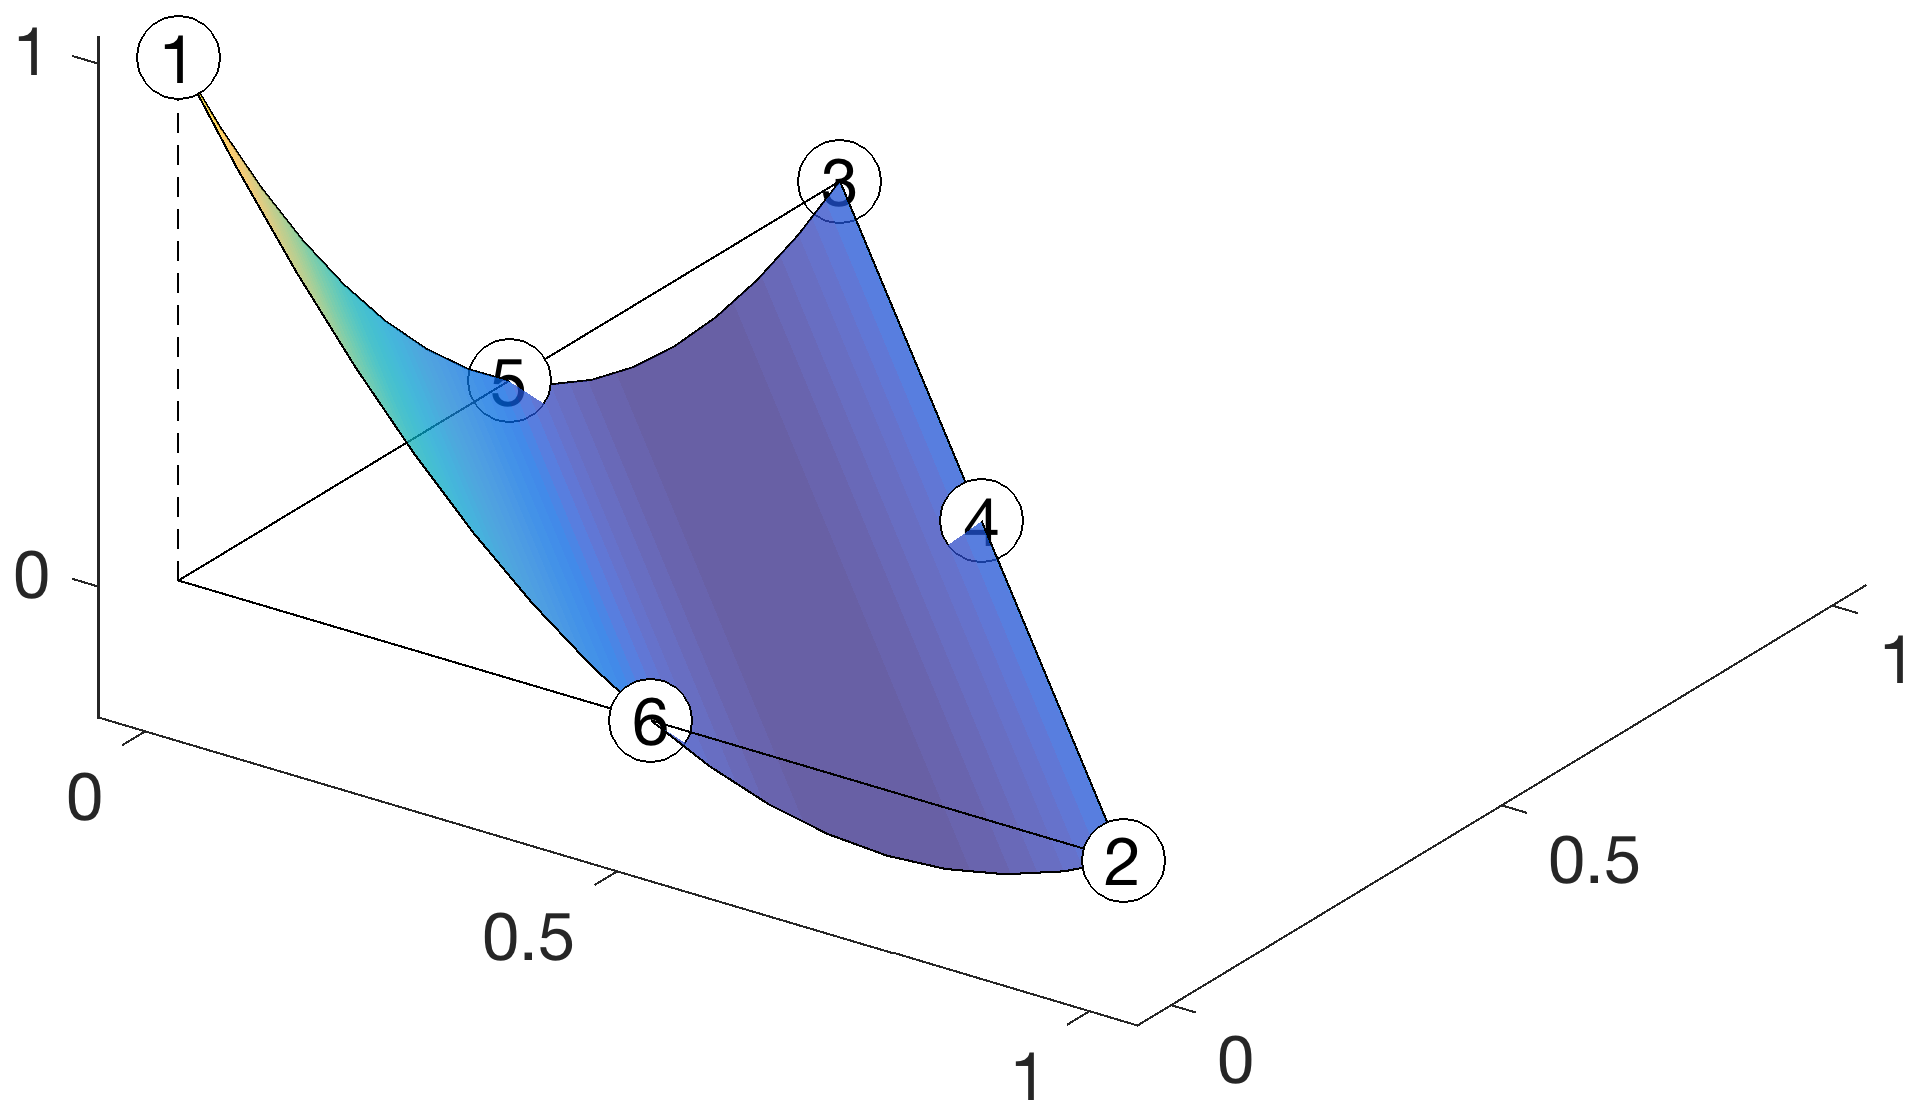
\includegraphics[width=0.3\textwidth]{shape_tri_p2_1}
  }
  \subfigure[$\tilde \phi_2$]{
    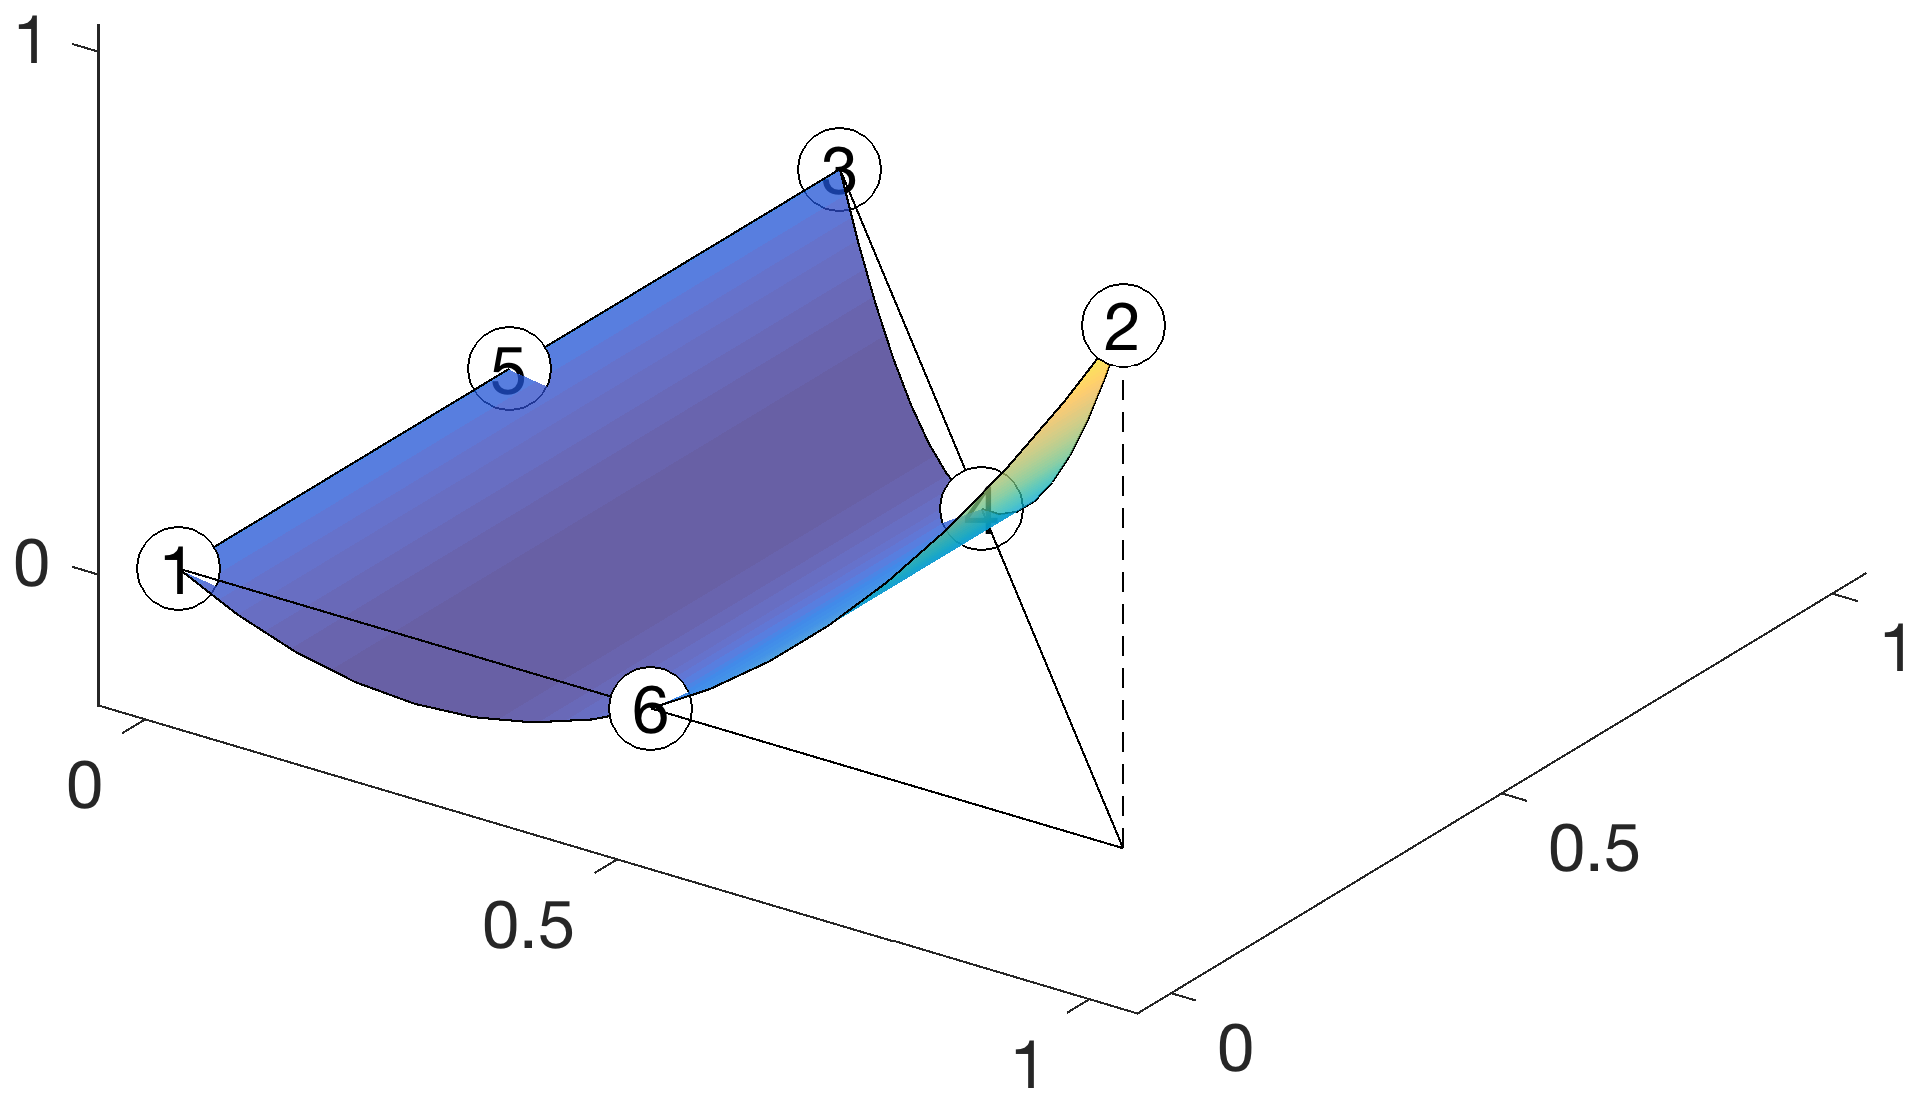
\includegraphics[width=0.3\textwidth]{shape_tri_p2_2}
  }
  \subfigure[$\tilde \phi_3$]{
    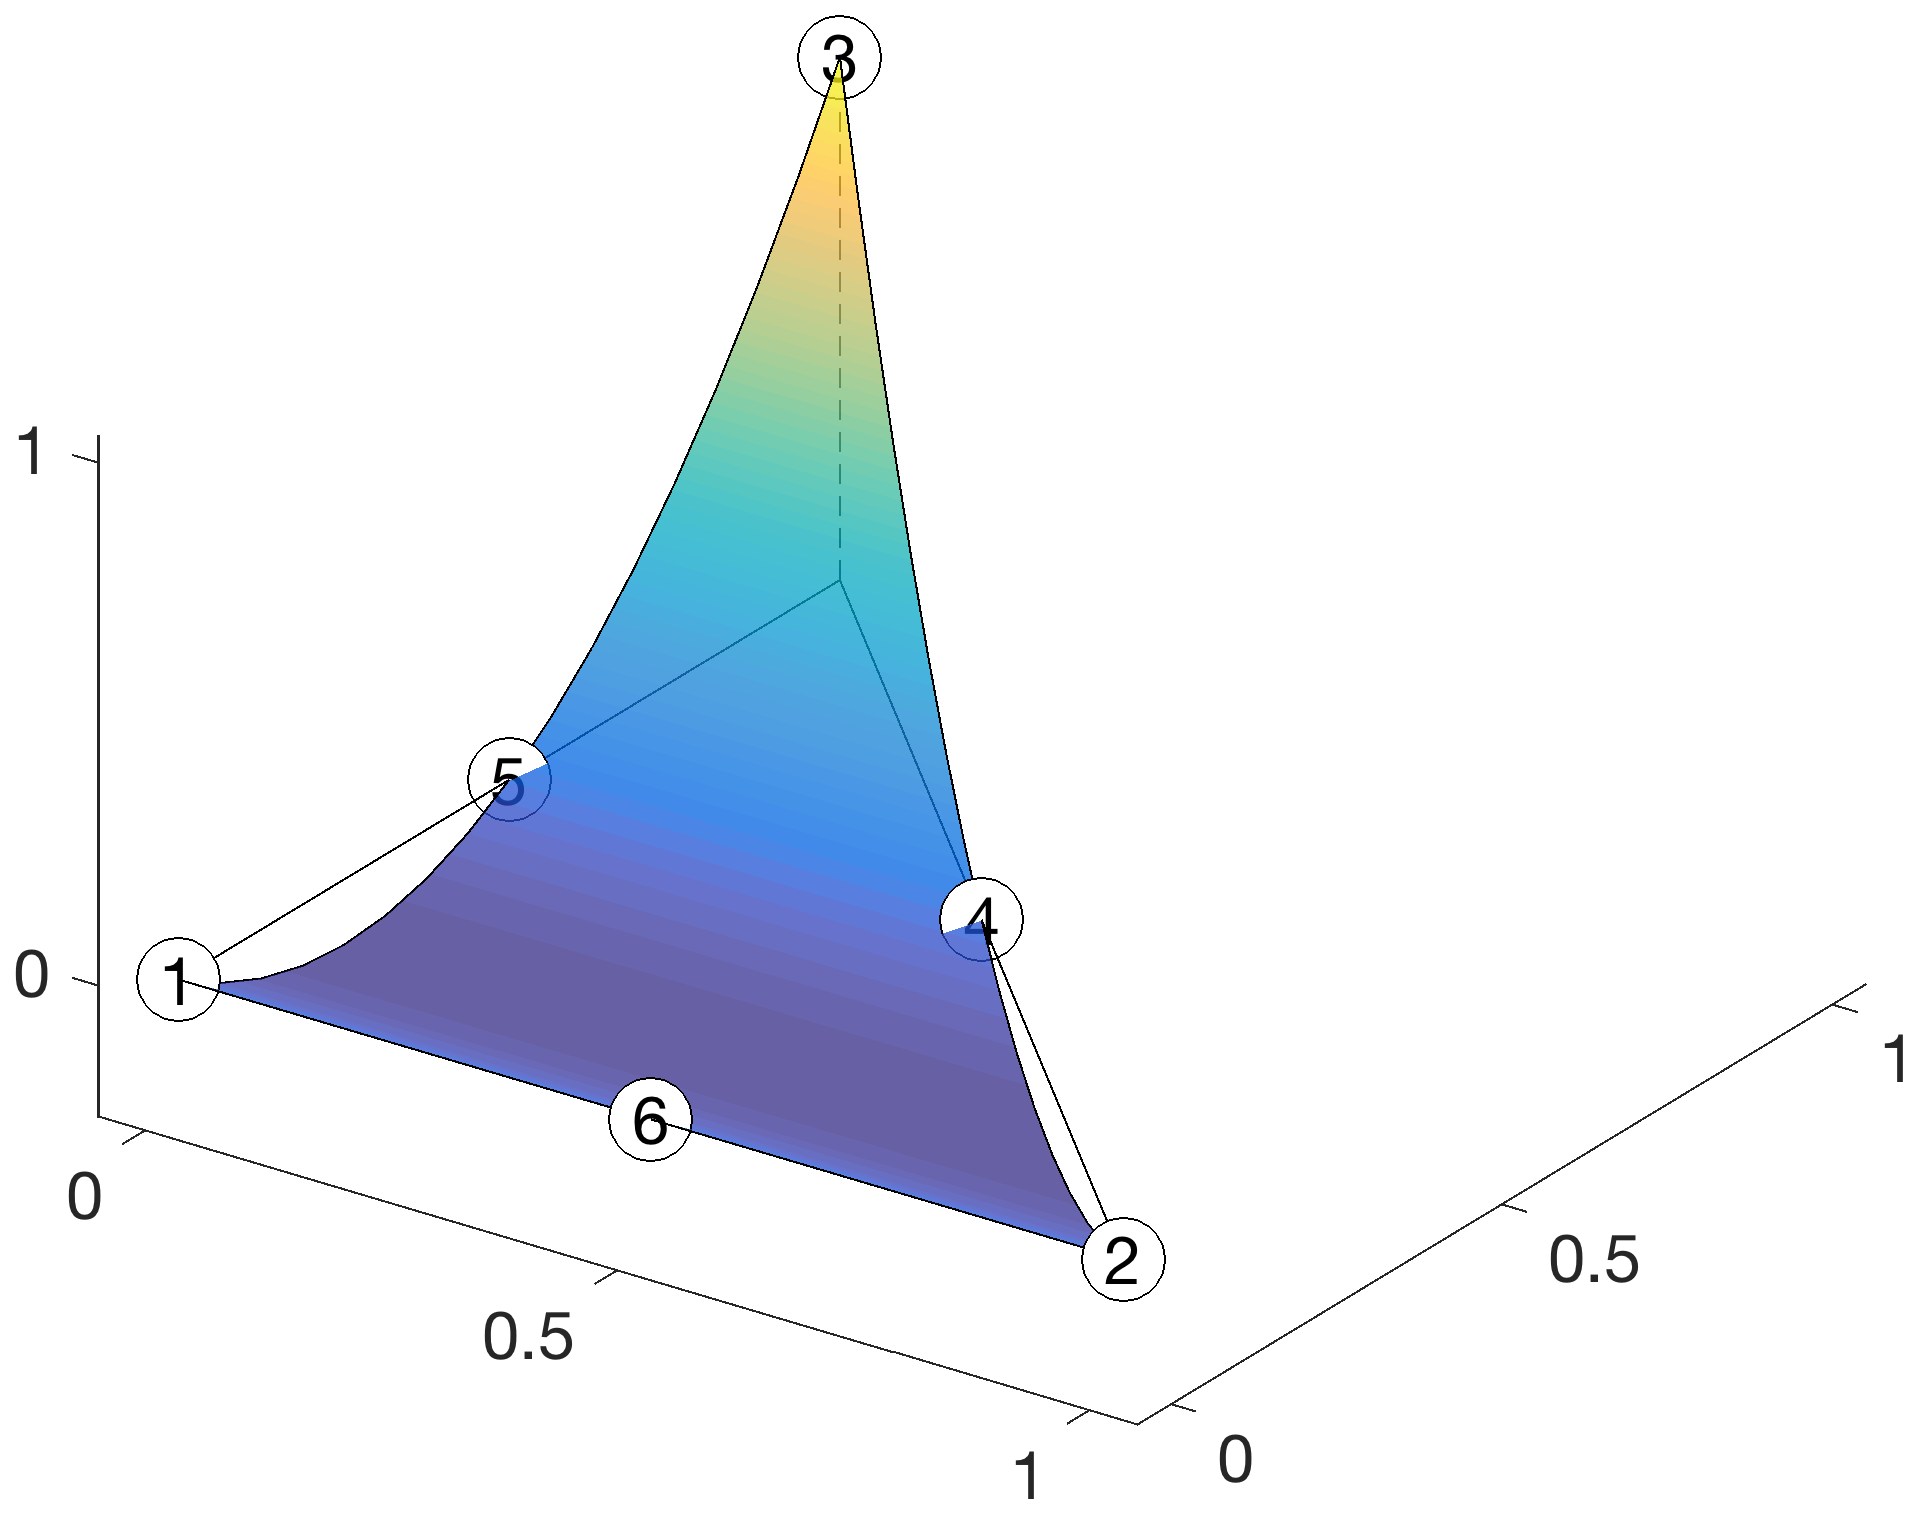
\includegraphics[width=0.3\textwidth]{shape_tri_p2_3}
  }
  \subfigure[$\tilde \phi_4$]{
    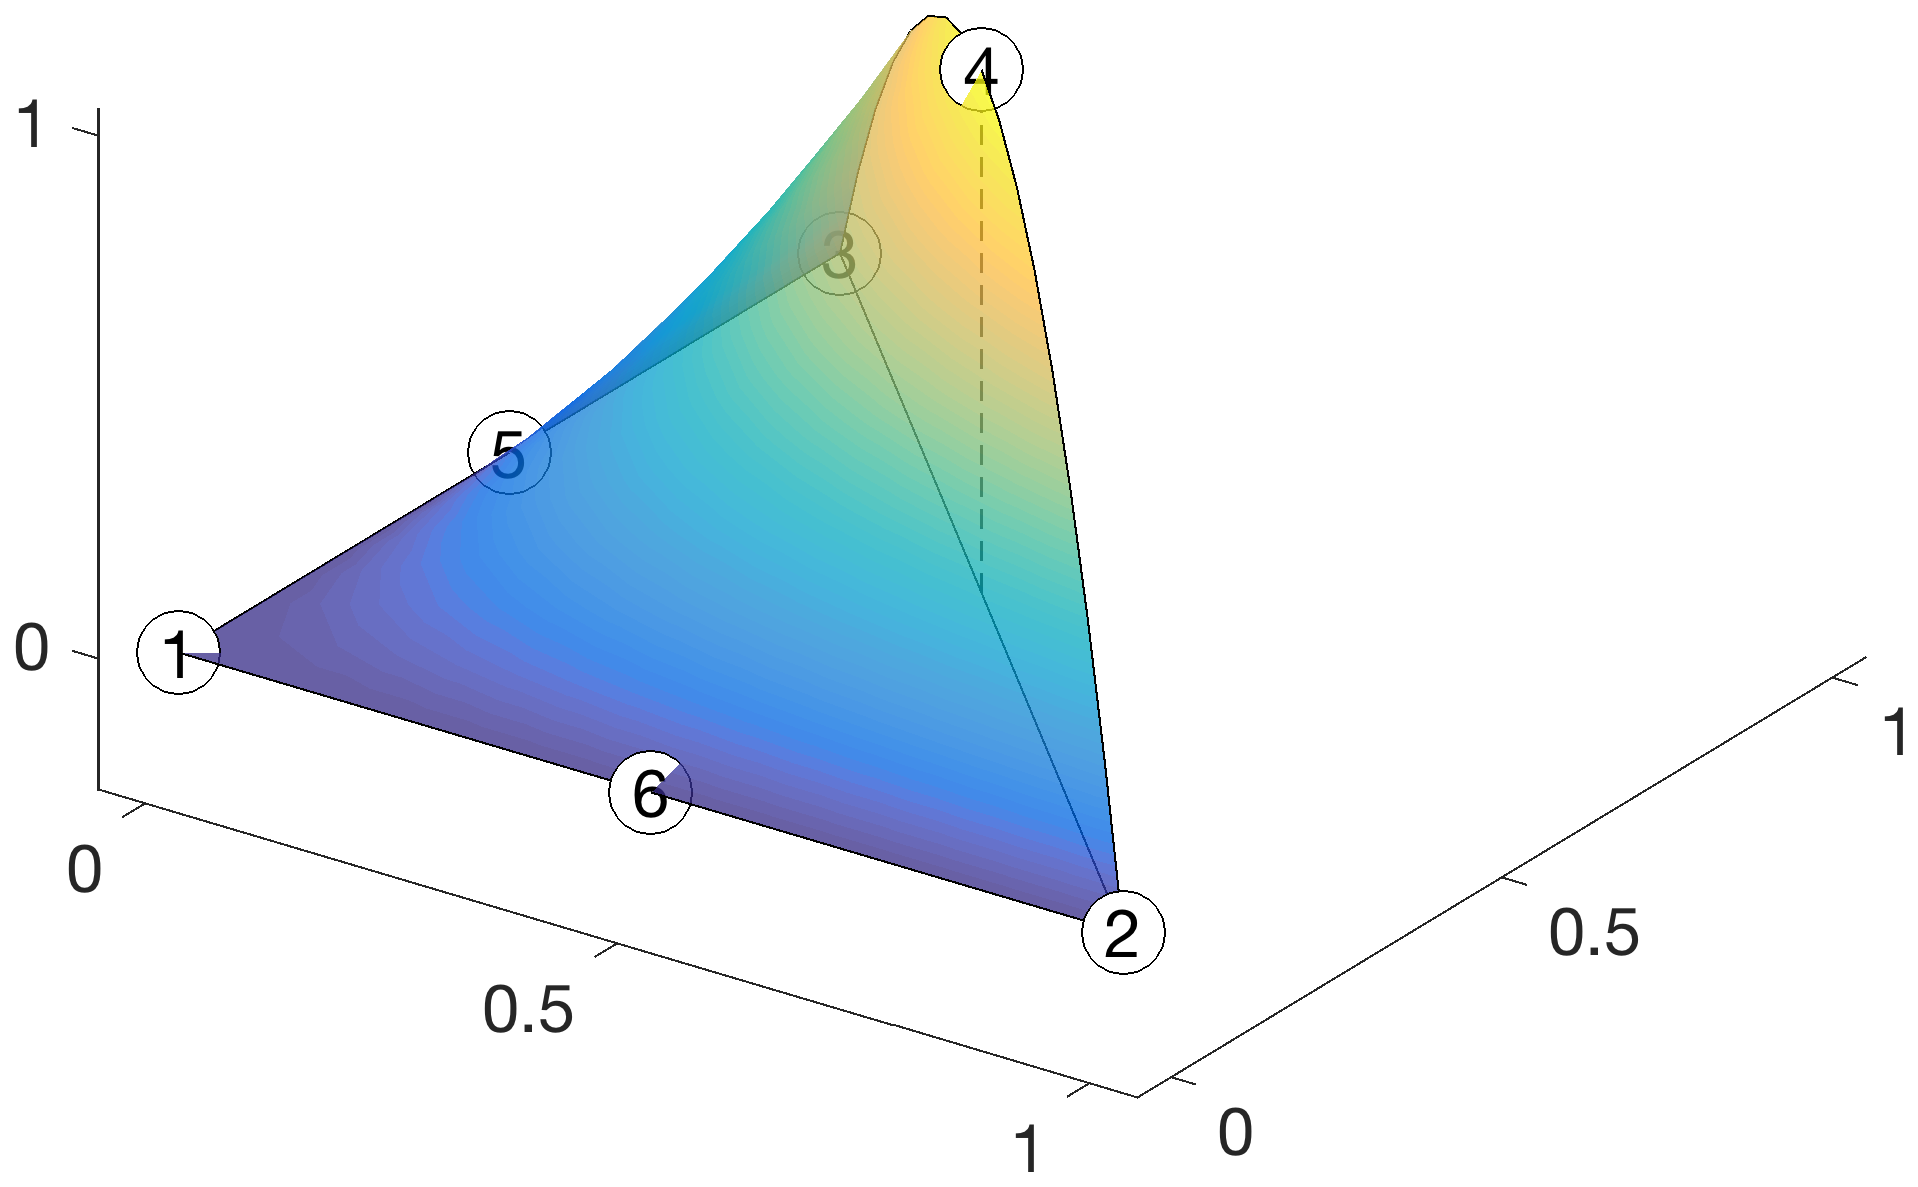
\includegraphics[width=0.3\textwidth]{shape_tri_p2_4}
  }
  \subfigure[$\tilde \phi_5$]{
    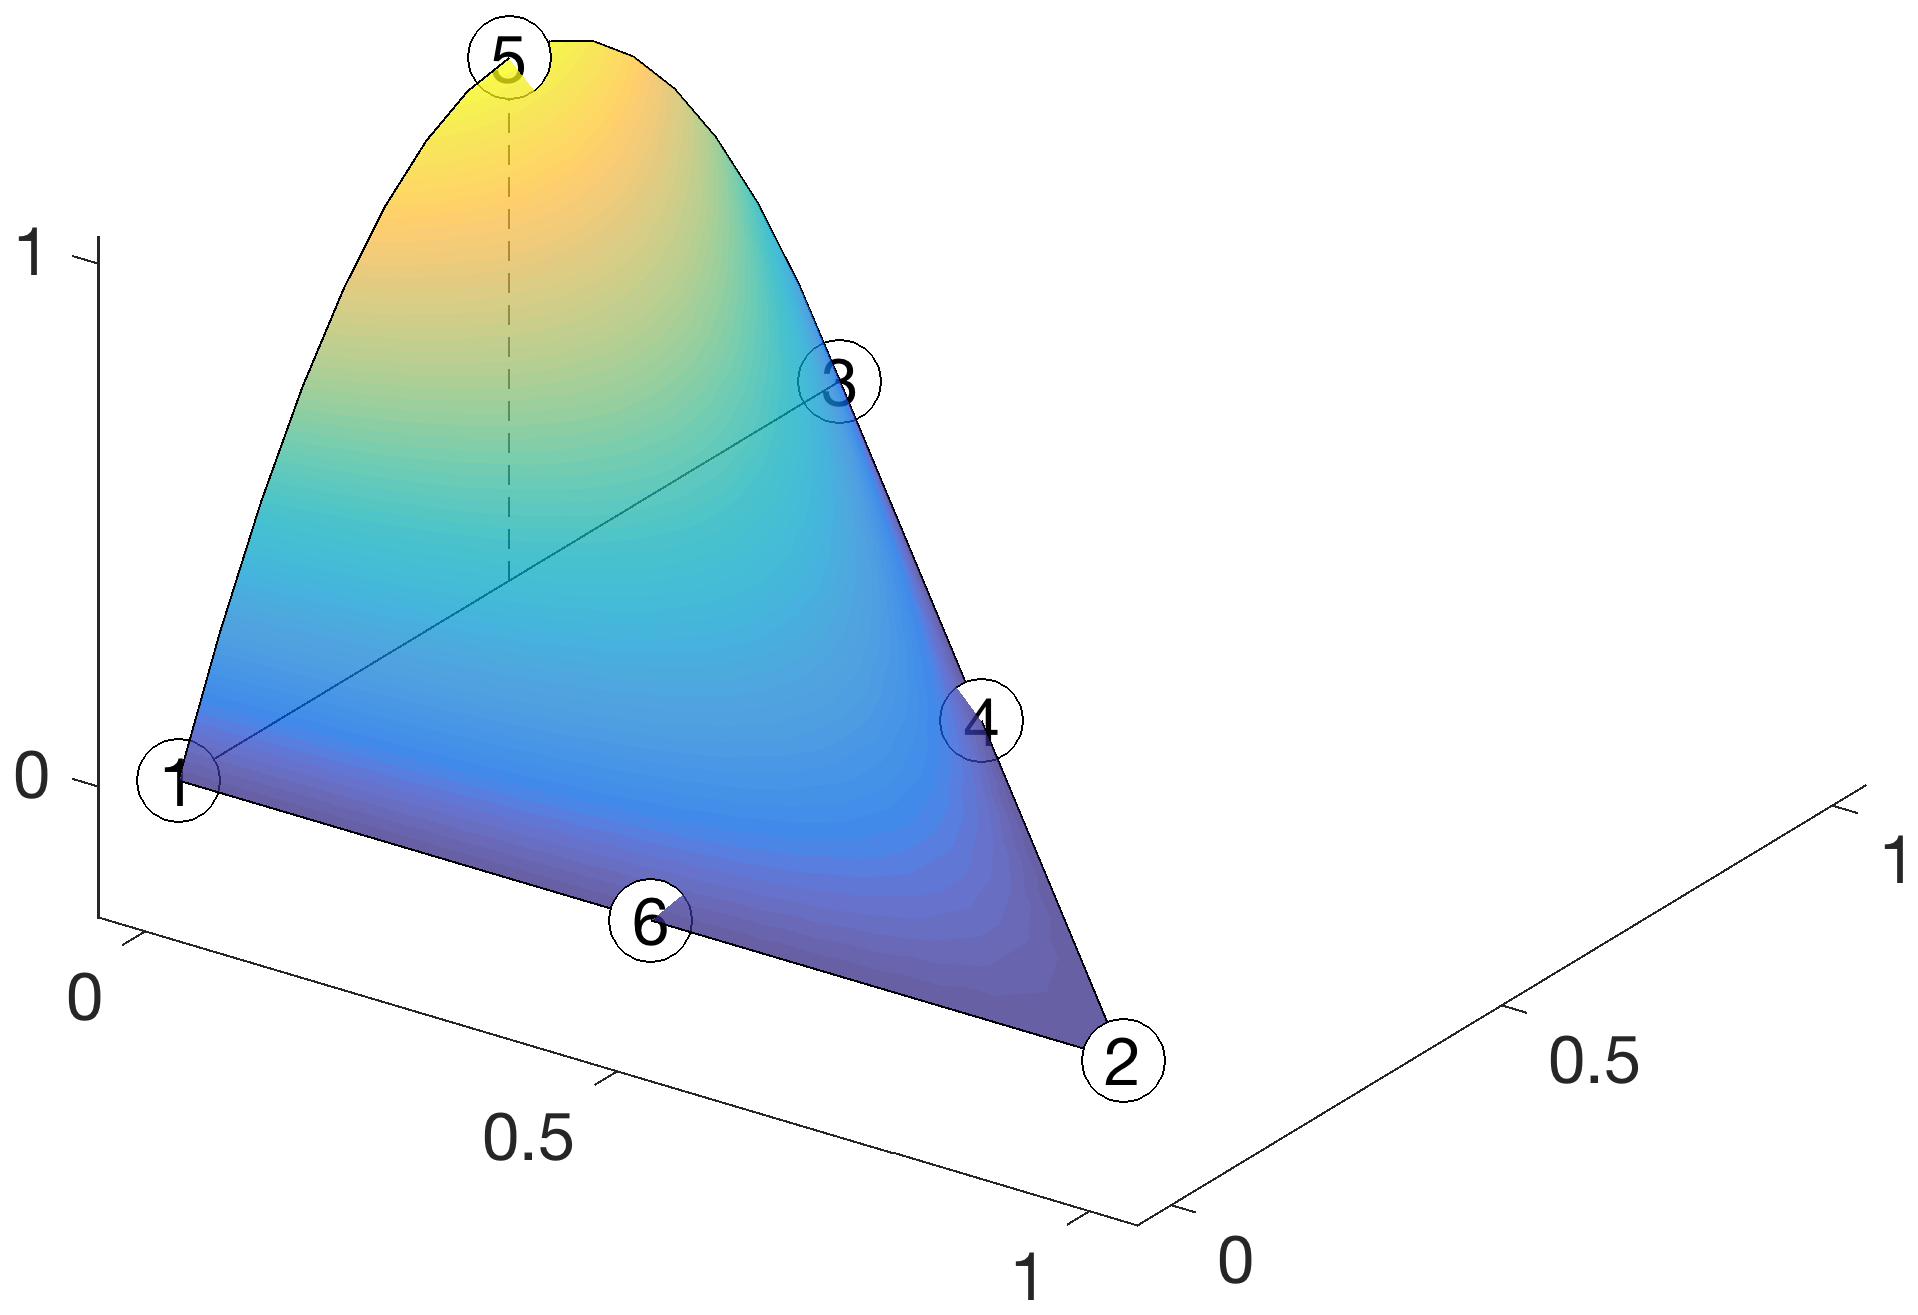
\includegraphics[width=0.3\textwidth]{shape_tri_p2_5}
  }
  \subfigure[$\tilde \phi_6$]{
    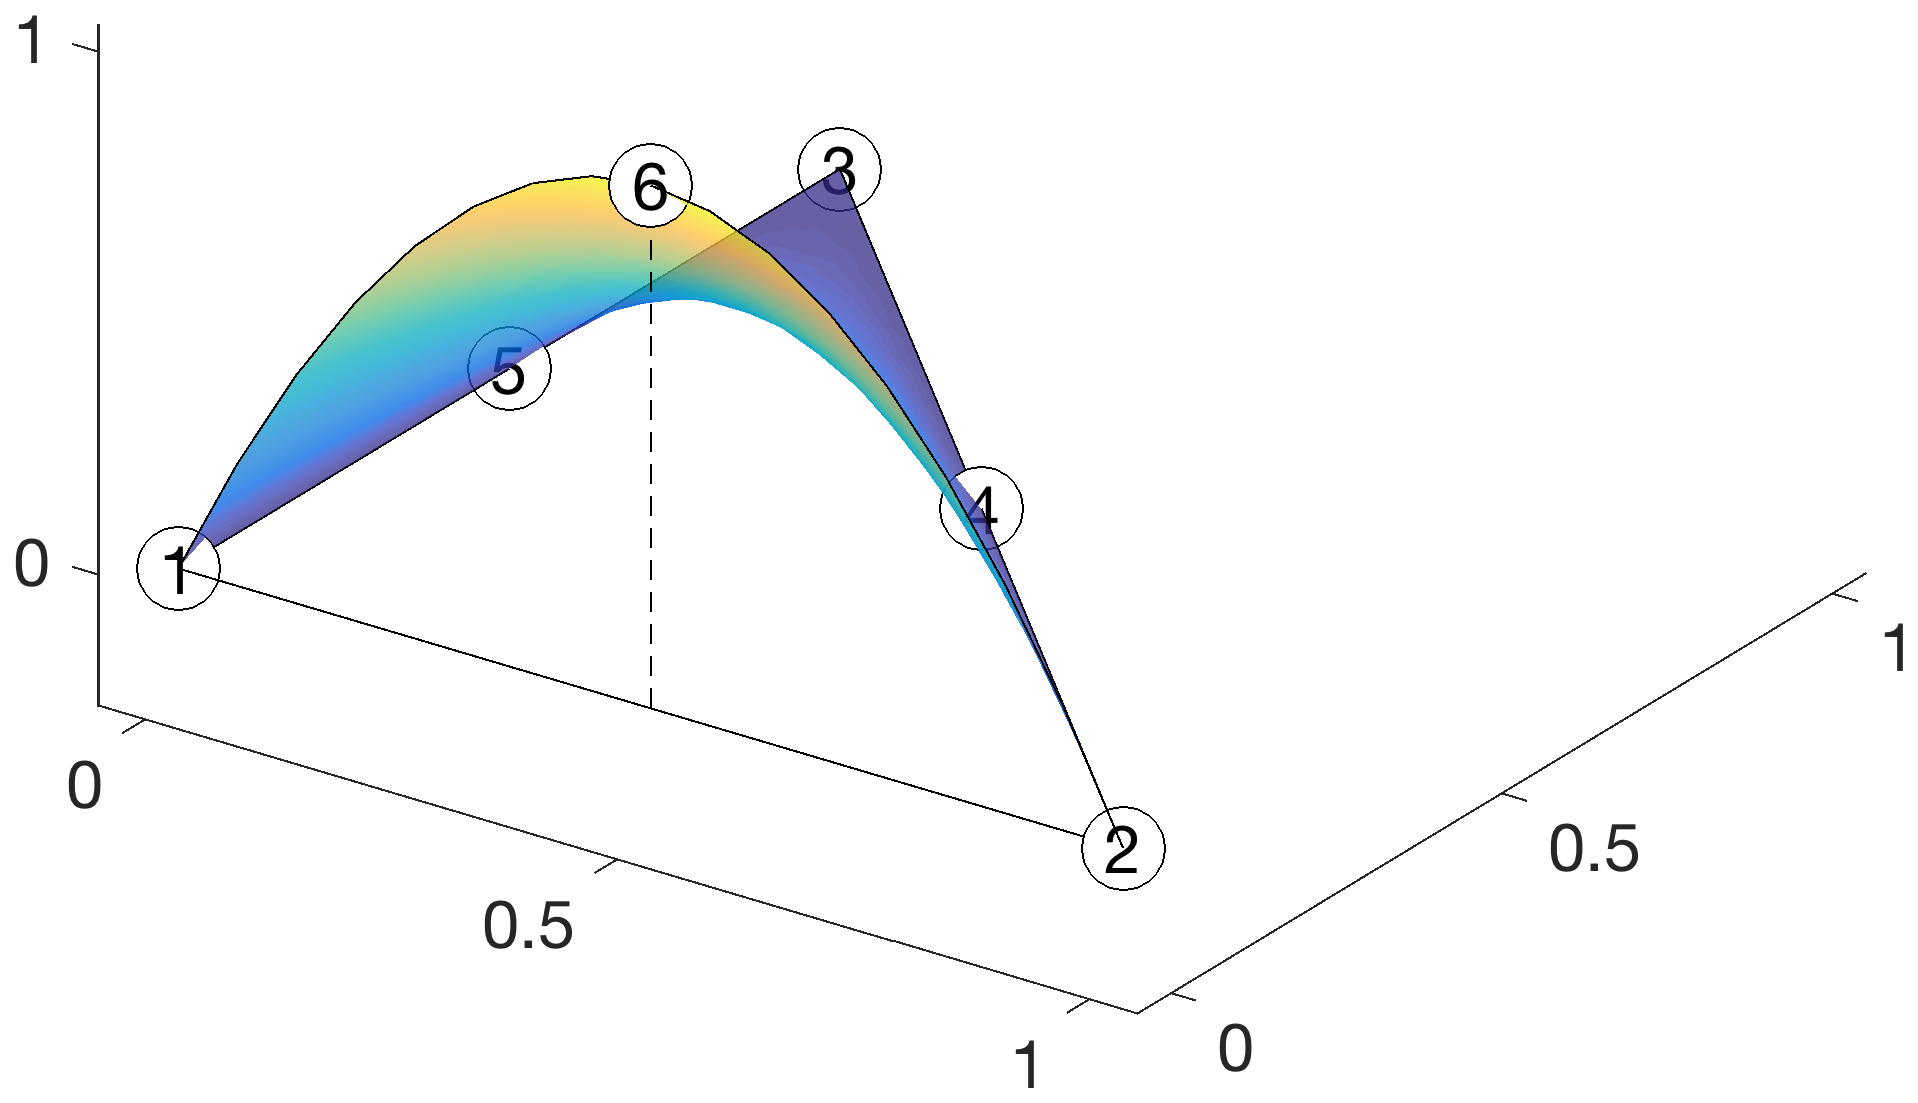
\includegraphics[width=0.3\textwidth]{shape_tri_p2_6}
  }
  \caption{Quadratic Lagrange shape functions on the reference triangle.}
  \label{fig:fe_shape_tri_p2}
\end{figure}

Once we find the coefficients of the basis functions, we can evaluate~\eqref{eq:fe_quad_tri_rep} to obtain the value of the basis function at any point in the reference triangle.  We can also differentiate~\eqref{eq:fe_quad_tri_rep} to obtain the gradient of the shape functions:
\begin{align*}
  \pp{\tilde \phi_j}{\tilde x_1} &= a^{(j)}_2 + 2 a^{(j)}_4 \tilde x^2_1 + a^{(j)}_5 \tilde x_2
  \\
  \pp{\tilde \phi_j}{\tilde x_2} &= a^{(j)}_3 + a^{(j)}_5 \tilde x_1 + 2 a^{(j)}_6 \tilde x_2.
\end{align*}
For the quadratic Lagrange element, the derivatives are linear functions.

\section{Generation: Lagrange element of arbitrary degree on arbitrary domain}
We can generalize the procedure to generate Lagrange basis functions of an arbitrary degree on an arbitrary domain.  Say we wish to generate Lagrange basis for a polynomial space of degree $p$ with a dimension of $n_s$.  Then, we first identify \emph{any} basis 
\begin{align*}
  \tilde \phi_i = \sum_{j=1}^{n_s} a^i \psi_j
\end{align*}

\begin{align*}
  \bmat{ccc}
  \psi_1(\tilde x^1) & \cdots & \psi_{n_s}(\tilde x^1) \\
  \vdots & \ddots & \vdots \\
  \psi_{n_s}(\tilde x^1) & \cdots & \psi_{n_s}(\tilde x^{n_s}) 
  \emat
  \bmat{ccc}
  a^1_1 & \cdots & a^{n_s}_1 \\
  \vdots & \ddots & \vdots \\
  a^1_{n_s} & \cdots & a^{n_s}_{n_s}
  \emat
  =
  I_{n_s},
\end{align*}
where $I_{n_s}$ is the $n_s \times n_s$ identity matrix.

%% \section{Bilinear Lagrange element on a quadrilateral}
%% We now consider arguably the simplest basis function on quadrilaterals: bilinear Lagrange basis on a reference quadrilateral.  Our reference quadrilateral is a unit square that is delineated by vertices
%% \begin{equation*}
%%   x^1 = (0,0), \quad x^2 = (1,0), \quad x^3 = (0,1), \quad \text{and} \quad x^4 = (1,1).
%% \end{equation*}
%% In two dimensions, any bilinear function can be expressed as a linear combination of monomial basis $\{ 1, x_1, x_2, x_1 x_2 \}$, which, unlike the triangular case, includes the cross term. Our interpolation points are the four vertices of the quadrilateral $\{ x^1, x^2, x^3, x^4 \}$.  Our shape functions are given by 
%% \begin{equation}
%%   \phi_i(x) = a_1^i + a_2^i x_1 + a_3^i x_2 + a_4^i x_1 x_2, \quad i = 1,\dots,4,
%%   \label{eq:fe_lin_quad_rep}
%% \end{equation}
%% where the coefficients satisfy
%% \begin{equation*}
%%   \bmat{cccc}
%%   1 & x_1^1 & x_2^1 & x_1^1 x_2^1 \\
%%   1 & x_1^2 & x_2^2 & x_1^2 x_2^2 \\
%%   1 & x_1^3 & x_2^3 & x_1^3 x_2^3 \\
%%   1 & x_1^4 & x_2^4 & x_1^4 x_2^4 \\
%%   \emat
%%   \bmat{cccc}
%%   a_1^1 & a_1^2 & a_1^3 & a_1^4 \\
%%   a_2^1 & a_2^2 & a_2^3 & a_2^4 \\
%%   a_3^1 & a_3^2 & a_3^3 & a_3^4 \\
%%   a_4^1 & a_4^2 & a_4^3 & a_4^4 \\
%%   \emat
%%   =
%%   \bmat{cccc}
%%   1 & 0 & 0 & 0 \\
%%   0 & 1 & 0 & 0 \\
%%   0 & 0 & 1 & 0 \\
%%   0 & 0 & 0 & 1
%%   \emat.
%% \end{equation*}
%% Once we find the coefficients, we can evaluate the value of the shape function at any point in the quadrilateral by evaluating~\eqref{eq:fe_lin_quad_rep}. We can also differentiate~\eqref{eq:fe_lin_quad_rep} to obtain gradient of the shape functions:
%% \begin{equation*}
%%   \pp{\phi_i}{x_1}(x) = a_2^i + a_4^ix_2
%%   \quad \text{and} \quad
%%   \pp{\phi_i}{x_2}(x) = a_3^i + a_4^ix_1, \quad i = 1,\dots,4.
%% \end{equation*}
%% Unlike the linear shape functions for triangles, the gradient of the \emph{bi}linear shape functions for quadrilateral depends on the evaluation point.


%% Formally, a finite element is defined by a triplet $(K,\calP,\Sigma)$ where
%% \begin{itemize}
%% \item[(i)] $K$ defines the domain
%% \item[(ii)] $\calP$ defines the (finite-dimensional) linear space of functions over $K$
%% \item[(iii)] $\Sigma$ defines the degrees of freedom such that a function $v \in \calP$ is uniquely determined.
%% \end{itemize}
%% For instance, for the linear Lagrange element in Section~\ref{sec:fe_lin_tri} chooses (i) the triangle as the domain $K$, (ii) space of linear functions $\PP^1(K)$ as the function space $\calP$, and (iii) the values of the function at the vertices of the triangle as the degree of freedom $\Sigma$. 

%% In general, a Lagrange basis is uniquely determined by (i) the degree of polyno




\begin{figure}
  \centering
  \subfigure[vertex shape function]{
    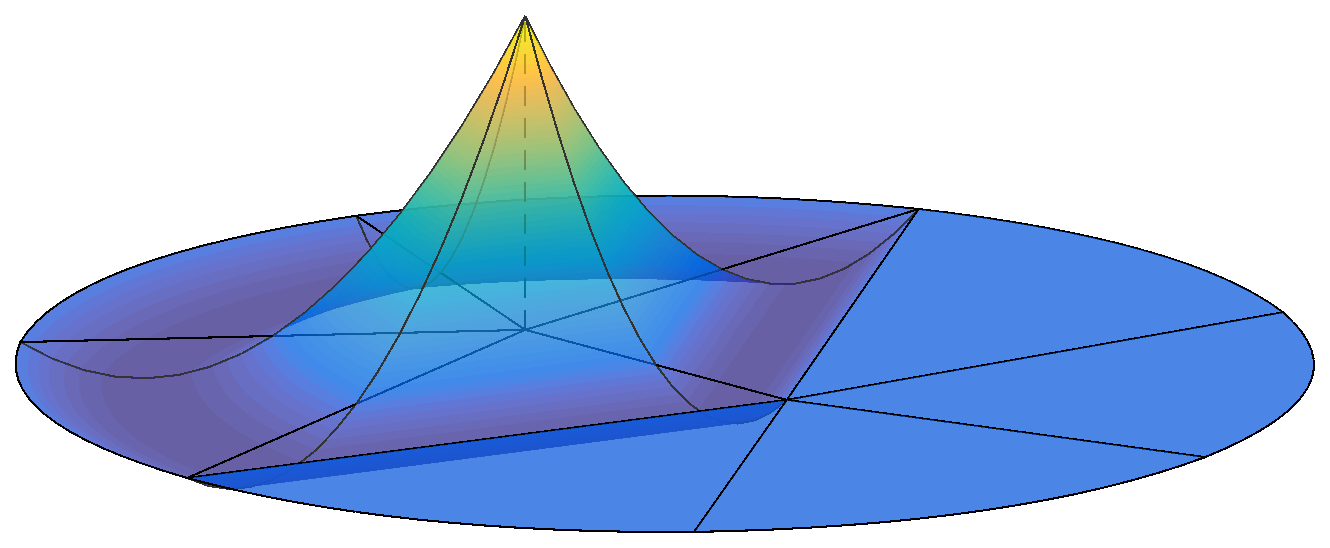
\includegraphics[width=0.48\textwidth]{shape_global_p2_1}
  }
  \subfigure[edge shape function]{
    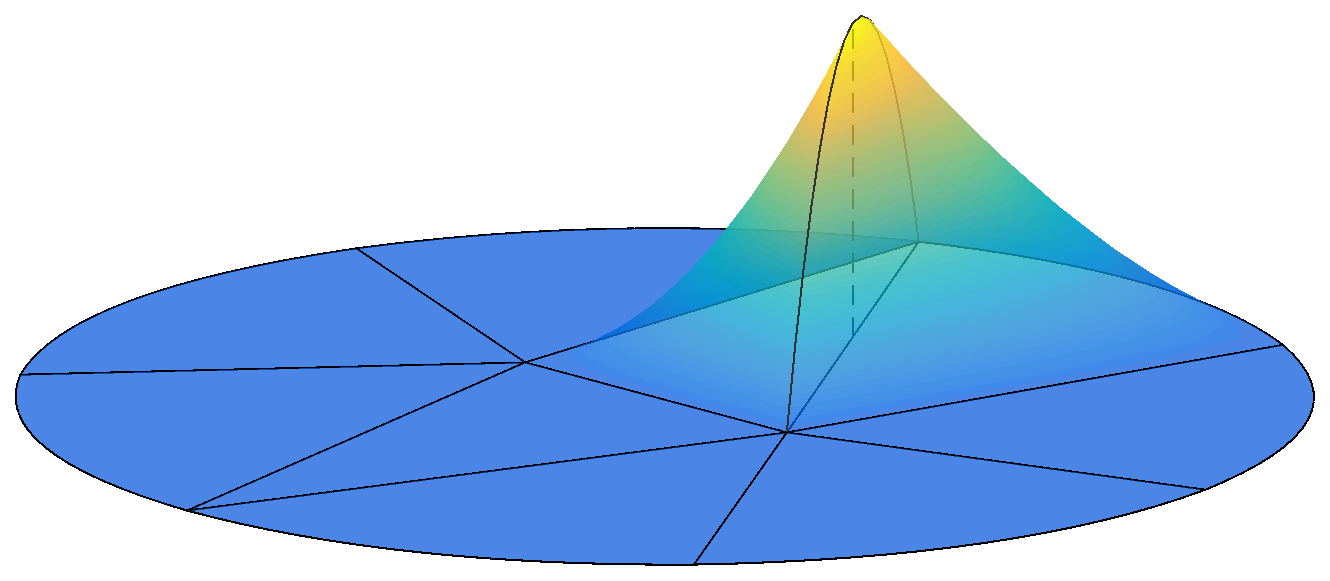
\includegraphics[width=0.48\textwidth]{shape_global_p2_2}
  }
\end{figure}


\begin{figure}
 \centering
 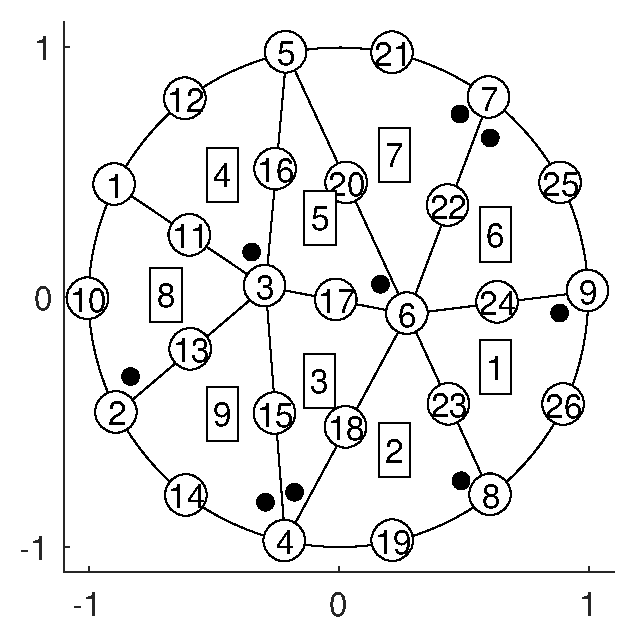
\includegraphics[width=0.4\textwidth]{fe_mesh_p2}
\end{figure}
\begin{table}
  \centering
  \subfigure[coordinates]{
    \begin{tabular}{c|cc}
      node & $x_1$ & $x_2$ \\
      \hline
      $1$ & $0.00$ & $0.67$ \\ 
      $2$ & $0.00$ & $0.00$ \\ 
      $3$ & $0.00$ & $1.00$ \\ 
      $4$ & $0.00$ & $0.34$ \\ 
      $5$ & $0.32$ & $0.00$ \\ 
      $6$ & $0.33$ & $1.00$ \\ 
      $7$ & $0.33$ & $0.66$ \\ 
      $8$ & $0.43$ & $0.31$ \\ 
      $9$ & $0.66$ & $1.00$ \\ 
      $10$ & $0.68$ & $0.00$ \\ 
      $11$ & $0.68$ & $0.58$ \\ 
      $12$ & $1.00$ & $0.68$ \\ 
      $13$ & $1.00$ & $0.33$ \\ 
      $14$ & $1.00$ & $0.00$ \\ 
      $15$ & $1.00$ & $1.00$ \\ 
      $16$ & $0.00$ & $0.84$ \\ 
      $17$ & $0.00$ & $0.50$ \\ 
      $18$ & $0.17$ & $0.84$ \\ 
      $19$ & $0.17$ & $0.66$ \\ 
      $20$ & $0.00$ & $0.17$ \\ 
      $21$ & $0.16$ & $0.00$ \\ 
      $22$ & $0.17$ & $1.00$ \\ 
      $23$ & $0.16$ & $0.17$ \\ 
      $24$ & $0.17$ & $0.50$ \\ 
      $25$ & $0.22$ & $0.32$ \\ 
      $26$ & $0.37$ & $0.16$ \\ 
      $27$ & $0.50$ & $0.00$ \\ 
      $28$ & $0.33$ & $0.83$ \\ 
      $29$ & $0.50$ & $1.00$ \\ 
      $30$ & $0.38$ & $0.48$ \\ 
      $31$ & $0.50$ & $0.83$ \\ 
      $32$ & $0.51$ & $0.62$ \\ 
      $33$ & $0.55$ & $0.16$ \\ 
      $34$ & $0.56$ & $0.45$ \\ 
      $35$ & $0.72$ & $0.32$ \\ 
      $36$ & $0.67$ & $0.79$ \\ 
      $37$ & $0.83$ & $0.84$ \\ 
      $38$ & $0.83$ & $1.00$ \\ 
      $39$ & $0.84$ & $0.16$ \\ 
      $40$ & $0.84$ & $0.00$ \\ 
      $41$ & $0.84$ & $0.63$ \\ 
      $42$ & $0.84$ & $0.45$ \\ 
      $43$ & $1.00$ & $0.50$ \\ 
      $44$ & $1.00$ & $0.84$ \\ 
      $45$ & $1.00$ & $0.16$ \\  
    \end{tabular}
  }
  \subfigure[connectivity]{
    \begin{tabular}{c|cccccc}
      element & node 1 & node 2 & node 3 \\
      \hline
      $1$ & $8$ & $13$ & $11$ & $42$ & $34$ & $35$ \\ 
      $2$ & $11$ & $13$ & $12$ & $43$ & $41$ & $42$ \\ 
      $3$ & $15$ & $9$ & $12$ & $37$ & $44$ & $38$ \\ 
      $4$ & $12$ & $9$ & $11$ & $36$ & $41$ & $37$ \\ 
      $5$ & $2$ & $5$ & $4$ & $23$ & $20$ & $21$ \\ 
      $6$ & $4$ & $5$ & $8$ & $26$ & $25$ & $23$ \\ 
      $7$ & $7$ & $8$ & $11$ & $34$ & $32$ & $30$ \\ 
      $8$ & $11$ & $9$ & $7$ & $31$ & $32$ & $36$ \\ 
      $9$ & $1$ & $4$ & $7$ & $24$ & $19$ & $17$ \\ 
      $10$ & $7$ & $4$ & $8$ & $25$ & $30$ & $24$ \\ 
      $11$ & $8$ & $5$ & $10$ & $27$ & $33$ & $26$ \\ 
      $12$ & $14$ & $13$ & $10$ & $39$ & $40$ & $45$ \\ 
      $13$ & $13$ & $8$ & $10$ & $33$ & $39$ & $35$ \\ 
      $14$ & $6$ & $7$ & $9$ & $31$ & $29$ & $28$ \\ 
      $15$ & $6$ & $3$ & $1$ & $16$ & $18$ & $22$ \\ 
      $16$ & $1$ & $7$ & $6$ & $28$ & $18$ & $19$ \\
    \end{tabular}
  }
\end{table}



\section{Interpolation error: linear element in one dimension}
\label{sec:fe_interp_1d}
In this section, we analyze the error associated with the piecewise linear interpolation of functions in one dimension. By way of preliminary, we first provide the definition of \emph{interpolant}.
\begin{definition}[interpolant]
Given $w \in \calV$, an interpolant $\calI_h w$ is an element of $\calV_h$ that satisfies the interpolation condition
\begin{equation*}
  (\calI_h w)(x_i) = w(x_i) \quad i = 1,\dots, N,
\end{equation*}
where $\{x_i \}_{i=1}^N$ is the set of interpolation points.
\end{definition}

We now focus on the piecewise linear space in one dimension.  To this end, given $\Omega \subset \RR$, we introduce an approximation space
\begin{equation*}
  \calV_h = \{ v \in \calV \ | \ v|_K \in \PP^1(K), \ \forall K \in \calT_h \}.
\end{equation*}

\begin{lemma}[One-dimensional linear interpolation error bound for $K$]
  Let $K \equiv [a,b]$ be the domain of length $h \equiv b - a$, $w \in C^2(K)$ be a function we wish to interpolate, and $\calI_h w \in \PP^1(K)$ be the linear interpolant based on the interpolation points $\{a,b\}$. Then, the interpolation error satisfies
  \begin{align}
    \| w - \calI_h w \|_{L^2(K)} &\leq \frac{1}{2} h^{5/2} \| w'' \|_{L^\infty(K)} \label{eq:fe_interp_lin_l2_elem} \\
    | w - \calI_h w |_{H^1(K)} &\leq h^{3/2} \| w '' \|_{L^\infty(K)}. \label{eq:fe_interp_lin_h1_elem}
  \end{align}
  \begin{proof}
    We first introduce an auxiliary function
    \begin{equation*}
      g(s) \equiv (w - \calI_hw)(s) - \left(
      \frac{(w - \calI_h w)(x)}{(x - a)(x-b)}
      \right)(s - a)(s-b).
    \end{equation*}
  We note that $g(x) = g(a) = g(b) = 0$ by construction. Hence $g$ has at least three roots in $K \equiv[a,b]$.  By Rolle's theorem, $g'$ has at least two roots in $K$.  Invoking Rolle's theorem one more time, we conclude that $g''$ has at least one root in $K$; let $\xi \in K$ be one of the roots of $g''$: i.e., $g''(\xi) = 0$.  We now compute the second derivative of $g$:
  \begin{equation*}
    g''(s) = w''(s) - \left(
      \frac{(w - \calI_h w)(x)}{(x - a)(x-b)}
      \right) \cdot 2;
  \end{equation*}
  note that $(\calI_h w)'' = 0$ since $\calI_h w$ is a linear function.  We now evaluate the expression at $\xi$ to obtain
  \begin{equation*}
    0 = w''(\xi) - \left(
      \frac{(w - \calI_h w)(x)}{(x - a)(x-b)}
      \right) \cdot 2, \quad \forall x \in K
  \end{equation*}
  or, equivalently,
  \begin{equation*}
    (w - \calI_h w)(x) = \frac{1}{2} w''(\xi) (x - a)(x - b).
  \end{equation*}
  The $L^2$ error bound follows from
  \begin{align*}
    \| w - \calI_h w \|^2_{L^2(K)}
    &= \int_K (w - \calI_h w)^2 dx
    = \frac{1}{4} \int_K w''(\xi)^2 (x-a)^2 (x-b)^2 dx
    \\
    &\leq\frac{1}{4} \| w'' \|_{L^\infty(K)}^2 \int_K (x-a)^2(x-b)^2 dx
    \leq \frac{1}{4} h^5 \| w'' \|_{L^\infty(K)}^2,
  \end{align*}
  where the inequality follows from $|x-a| < h$ and $|x-b| < h$.  To obtain the $H^1$ error bound, we first note
  \begin{equation*}
    (w - \calI_hw)'(x) = \frac{1}{2} w''(\xi) ((x-a) + (x-b));
  \end{equation*}
  it thus follows
  \begin{align*}
    | w - \calI_h w |^2_{H^1(K)}
    &= \int_K ((w - \calI_h w)')^2 dx
    = \int_K w''(\xi)^2 \frac{1}{4} ((x-a) + (x-b))^2 dx
    \\
    &\leq \| w'' \|_{L^\infty(K)}^2 \int_K \frac{1}{4} ((x-a) + (x-b))^2 dx
    \leq h^3\| w'' \|_{L^2(K)}^2,
  \end{align*}
  where the inequality again follows from $|x - a| < h$ and $|x - b| < h$.
    \end{proof}
\end{lemma}

\begin{proposition}[One-dimensional linear interpolation error bound for $\Omega$]
  Let $\Omega \subset \RR^1$ be the domain, $\calT_h$ be a uniform triangulation over $\Omega$ of characteristic length $h$, $w \in \oplus_{K \in \calT_h}  C^2(K)$ be a function we wish to interpolate, and $\calI_h w \in \calV_h$ be the linear interpolant associated with $\calV_h \equiv \{ v \in C^0(\Omega) \ | \ v|_K \in \PP^1(K), \ \forall K \in \calT_h \}$. Then, the interpolation error satisfies
  \begin{align}
    \| w - \calI_h w \|_{L^2(\Omega)} &\leq \frac{1}{2} h^2 \| w'' \|_{L^\infty(\Omega)} \label{eq:fe_interp_lin_l2} \\
    | w - \calI_h w |_{H^1(\Omega)} &\leq h \| w'' \|_{L^\infty(\Omega)} \label{eq:fe_interp_lin_h1}
  \end{align}
  \begin{proof}
    The $L^2$ error bound follows from the application of~\eqref{eq:fe_interp_lin_l2_elem} to each element:
    \begin{equation*}
      \| w - \calI_h w \|^2_{L^2(\Omega)}
      =
      \sum_{K \in \calT_h} \| w - \calI_h w \|^2_{L^2(K)}
      \leq
      \frac{1}{h} \frac{1}{4} h^5 \| w'' \|_{L^\infty(\Omega)}^2
      = \frac{1}{4} h^4 \| w'' \|_{L^\infty(\Omega)}^2.
    \end{equation*}
    The $H^1$ error bound similarly follows from the application of~\eqref{eq:fe_interp_lin_h1_elem} to each element:
        \begin{equation*}
      \| w - \calI_h w \|^2_{L^2(\Omega)}
      =
      \sum_{K \in \calT_h} \| w - \calI_h w \|^2_{L^2(K)}
      \leq
      \frac{1}{h} h^3 \| w'' \|_{L^\infty(\Omega)}^2
      = h^2 \| w'' \|_{L^\infty(\Omega)}^2.
    \end{equation*}
  \end{proof}
\end{proposition}
The proposition shows that the $L^2$ interpolation error (i) depends on the maximum value of the second derivative $\| w '' \|_{L^\infty(\Omega)}$ and (ii) decreases as $h^2$.  The $H^1$ interpolation error similarly depends on $\| w'' \|_{L^\infty(\Omega)}$ but decreases as $h^1$. 

\section{Interpolation error: general polynomial interpolant}
The interpolation error bound obtained in Section~\ref{sec:fe_interp_1d} can be generalized to (i) higher dimensions, (ii) higher degree polynomials, and (iii) $H^k(\Omega)$ norm for $k \geq 0$.  However, the associated proof, which builds on the Bramble-Hilbert lemma, is beyond the scope of this lecture.  We here simply state the result.
\begin{proposition}
Let $w \in H^s(\Omega)$ be a function we wish to interpolate, $\calT_h$ be a triangulation of a characteristic diameter $h$, $\calI_h w \in \calV_h$ be the piecewise polynomial interpolant of degree $p$ associated with $\calT_h$. Then, the $L^2(\Omega)$ interpolation error satisfies
\begin{align*}
  \| w - \calI_h w \|_{L^2(\Omega)} \leq C h^{r+1} | w |_{H^{r+1}(\Omega)}
\end{align*}
for $r = \min\{ s,p \}$ and some $C$ independent of $h$. Similarly, for $k \geq 0$, the $H^k(\Omega)$ interpolation error satisfies 
\begin{align*}
  \| w - \calI_h w \|_{H^k(\Omega)} \leq C h^{r+1-k} | w |_{H^{r+1}(\Omega)}
\end{align*}
for $r = \min\{ s,p \}$ and some $C$ independent of $h$.
\end{proposition}



%i.e., for a piecewise polynomial space $\calV_h$,
%\begin{equation*}
%  \calV_h \subset \calV \quad \Leftrightarrow \quad \calV_h \subset C^0(\overline \Omega) ,
%\end{equation*}
%where  $C^0(\overline \Omega)$ is the space of continuous functions over $\overline \Omega$.

%Given the continuity requirement, we will construct finite element spaces of the form
%\begin{equation}
%  \calV_h \equiv \{ v \in C^0(\overline \Omega) \ | v |_{K_i} \in \PP^p(K_i), \ i = 1,\dots, n_e \};
%  \label{eq:fe_space}
%\end{equation}
%we recall that $\PP^p(K_i)$ is the space of degree $p$ polynomials over $K_i$.





%% \section{Linear Lagrange element on a line segment}
%% \label{sec:fe_lin_line}
%% We first introduce arguably the simplest finite element: linear Lagrange element on a unit line segment $\tilde K$.  Our unit line segment $\tilde K \equiv (\tilde x^1, \tilde x^2)$ is delineated by two endpoints
%% \begin{equation*}
%%   \tilde x^1 = 0 \quad \text{and} \quad \tilde x^2 = 1.
%% \end{equation*}
%% For the linear polynomial space $\PP^1(\tilde K)$ and the interpolation points $\{\tilde x^1, \tilde x^2\}$, a unique set of \emph{Lagrange basis functions} (or \emph{Lagrange shape functions}) is given by
%% \begin{equation*}
%%   \tilde \phi_1(\tilde x) = 1 - \tilde x \quad \text{and} \quad \tilde \phi_2(\tilde x) = \tilde x.
%% \end{equation*}
%% Note that these basis functions satisfy the interpolation condition
%% \begin{equation*}
%%   \phi_i(\tilde x^j) = \delta_{ij}.
%% \end{equation*}
%% Here $\delta_{ij}$ is the \emph{Kronecker delta}: $\delta_{ij} = 1$ for $i = j$ and $\delta_{ij} = 0$ for $i \neq j$.

%% With these basis functions, we can describe any function $v \in \PP^1(\tilde K)$ as
%% \begin{equation*}
%%   v = \sum_{i=1}^{n_s} \tilde v_i \tilde \phi_i
%% \end{equation*}
%% for $\tilde v_i \equiv v(\tilde x^i)$, $i = 1,2$; the values of the function at the end points are the degree of freedom of the finite element.  Similarly, the derivative of the function is given by
%% \begin{equation*}
%%   \pp{v}{\tilde x} = \sum_{i=1}^{n_s} \tilde v_i \pp{\tilde \phi_i}{\tilde x},
%% \end{equation*}
%% where the direct differentiation of the basis functions yields $\pp{\tilde \phi_1}{\tilde x} = -1$ and $\pp{\tilde \phi_2}{\tilde x} = 1$.


%To see the equivalence, we observe that .  Conversely, if a polynomial space is no
%We hence choose
%\begin{equation*}
%  \calV_h \equiv \{ v \in C^0(\overline \Omega) \ | v |_{K_i} \in \PP^p(K_i), \ i = 1,\dots, n_e \};
%\end{equation*}
%



%% \section{Linear Lagrange finite element on line segments}


%% \label{sec:fe_lin_line}
%% We first introduce arguably the simplest form of finite element: linear Lagrange elements on (one-dimensional) line. In one dimension, any linear function can be expressed as a linear combination of a monomial basis
%% \begin{equation*}
%%   \{ 1, x \};
%% \end{equation*}
%% by construction, $\text{span}\{1,x\} = \PP^1(K)$. Our goal is to find the \emph{Lagrange shape functions}
%% \begin{equation*}
%%   \{ \phi_1, \phi_2 \}
%% \end{equation*}
%% that forms a basis (i.e., $\text{span}\{ \phi_1, \phi_2 \} = \PP^1(K)$) and satisfies the interpolation condition
%% \begin{equation}
%%   \phi_i(x^j) = \delta_{ij};  \label{eq:fe_interp}
%%  % \equiv
%%  % \begin{cases}
%%  %   1, \quad i = j \\
%%  %   0, \quad i \neq j
%%  % \end{cases} 
%% \end{equation}
%% here $\delta_{ij}$ is the \emph{Kronecker delta} such that $\delta_{ij} = 1$ for $i = j$ and $\delta_{ij} = 0$ for $i \neq j$.  To find the basis, we first express the shape functions in terms of the monomial basis:
%% \begin{equation}
%%   \phi_i(x) = a^i_1 + a^i_2 x \quad i = 1, 2.
%%   \label{eq:fe_lin_line_rep}
%% \end{equation}
%% We now apply the interpolation condition~\eqref{eq:fe_interp} to find the coefficients.  For instance, $\phi_1$ must satisfy
%% \begin{equation*}
%%   \bmat{cc}
%%   1 & x^1 \\
%%   1 & x^2 \\
%%   \emat
%%   \bmat{c}
%%   a_1^1 \\ a_2^1 
%%   \emat
%%   =
%%   \bmat{c}
%%   1 \\ 0 
%%   \emat
%% \end{equation*}
%% We can also pose a single matrix equation for the monomial coefficients of all three shape functions: 
%% \begin{equation*}
%%   \bmat{cc}
%%   1 & x^1 \\
%%   1 & x^2 \\
%%   \emat
%%   \bmat{cc}
%%   a_1^1 & a_1^2 \\
%%   a_2^1 & a_2^2 \\
%%   \emat
%%   =
%%   \bmat{cc}
%%   1 & 0 \\
%%   0 & 1 \\
%%   \emat.
%% \end{equation*}
%% We note that the matrix in the first matrix in the left hand side is the \emph{Vandermonde matrix} associated with our monomial basis evaluated at the vertices of the triangle.  The linear equation is well-posed as long as the interpolation points are not colinear, which is equivalent to the condition that the triangle have a finite area.

%% Once we find the coefficients of the shape functions, we can evaluate the value of the functions at any point in the triangle by evaluating~\eqref{eq:fe_lin_line_rep}. We can also differentiate~\eqref{eq:fe_lin_line_rep} to obtain the gradient of the shape functions:
%% \begin{align*}
%%   \pp{\phi_i}{x}(x) = a_2^i
%% \end{align*}
%% The derivatives are constant over the element because the shape functions are linear.
